% Nejprve uvedeme tridu dokumentu s volbami
\documentclass[czech,bachelor]{diploma}
% Dalsi doplnujici baliky maker
\usepackage[autostyle=true,czech=quotes]{csquotes} % korektni sazba uvozovek, podpora pro balik biblatex
\usepackage[backend=biber, style=iso-numeric, alldates=iso]{biblatex} % bibliografie
\usepackage{dcolumn} % sloupce tabulky s ciselnymi hodnotami
\usepackage{subfig} % makra pro "podobrazky" a "podtabulky"
\usepackage[cpp]{diplomalst}

%====================dockerfile=================================

\usepackage{color}
\usepackage{listings}
\usepackage{placeins} 
\usepackage{hyperref}
\usepackage{svg}
\usepackage{amsmath}



\lstdefinelanguage{Dockerfile}
{
  morekeywords={FROM, RUN, CMD, LABEL, MAINTAINER, EXPOSE, ENV, ADD, COPY,
    ENTRYPOINT, VOLUME, USER, WORKDIR, ARG, ONBUILD, STOPSIGNAL, HEALTHCHECK,
    SHELL},
  morecomment=[l]{\#},
  morestring=[b]"
}

\lstset{
    columns=flexible,
    keepspaces=true,
    showstringspaces=false,
    basicstyle=\small\ttfamily,
    basewidth= {.5em,0.4em},
    commentstyle=\color{gray},
    keywordstyle=\color{purple},
    stringstyle=\color[RGB]{163,60,80}
}
%====================dockerfile=================================

%====================json====================================
\colorlet{punct}{red!60!black}
\definecolor{background}{HTML}{EEEEEE}
\definecolor{delim}{RGB}{20,105,176}
\colorlet{numb}{magenta!60!black}

\lstdefinelanguage{json}{
    basicstyle=\normalfont\ttfamily,
    numbers=left,
    numberstyle=\scriptsize,
    stepnumber=1,
    numbersep=8pt,
    showstringspaces=false,
    breaklines=true,
    frame=lines,
    literate=
     *{0}{{{\color{numb}0}}}{1}
      {1}{{{\color{numb}1}}}{1}
      {2}{{{\color{numb}2}}}{1}
      {3}{{{\color{numb}3}}}{1}
      {4}{{{\color{numb}4}}}{1}
      {5}{{{\color{numb}5}}}{1}
      {6}{{{\color{numb}6}}}{1}
      {7}{{{\color{numb}7}}}{1}
      {8}{{{\color{numb}8}}}{1}
      {9}{{{\color{numb}9}}}{1}
      {:}{{{\color{punct}{:}}}}{1}
      {,}{{{\color{punct}{,}}}}{1}
      {\{}{{{\color{delim}{\{}}}}{1}
      {\}}{{{\color{delim}{\}}}}}{1}
      {[}{{{\color{delim}{[}}}}{1}
      {]}{{{\color{delim}{]}}}}{1},
}
%====================json====================================
\newcommand{\specialcell}[2][c]{%
  \begin{tabular}[#1]{@{}c@{}}#2\end{tabular}}
\newcolumntype{C}[1]{>{\centering}m{#1}}
  
% Zadame pozadovane vstupy pro generovani titulnich stran.
\ThesisAuthor{Jakub Konvička}

\ThesisSupervisor{Ing. Václav Svatoň, Ph.D.}

\CzechThesisTitle{HEAppE Middleware rozšíření pro lokální výpočty a uživatelsky definované šablony výpočtů}

\EnglishThesisTitle{HEAppE Middleware Extension for Local Computing and User Defined Command Templates}

\SubmissionYear{2022}

\ThesisAssignmentFileName{ThesisSpecification.pdf}

% Pokud nechceme nikomu dekovat makro zapoznamkujeme.
\Acknowledgement{Rád bych na tomto místě poděkoval vedoucímu bakalářské práce Ing. Václavu Svatoňovi, Ph.D. a Ing. Janu Křenkovi za jejich rady a čas, který mi věnovali při řešení dané problematiky.}

\CzechAbstract{Cílem této práce je návrh a následná implementace rozšíření Open-Source aplikačního frameworku HEAppE Middleware o podporu lokálního spouštění výpočetních úloh a rozšíření funkcionality middleware o správu uživatelsky definovaných šablon výpočtů, které se využívají při specifikaci HPC úloh. HEAppE Middleware je systém implementující koncept HPC-as-a-Service, uživatelům poskytuje rozhraní ke správě HPC úloh a přístupu k jejich datům na superpočítačových clusterech.}

\CzechKeywords{High-performance computing, HPC-as-a-Service, HEAppE Middleware, výpočetní cluster}

\EnglishAbstract{The purpose of this thesis is to design and then implement an extension of the Open-Source application framework HEAppE Middleware to support local execution of computational tasks and to extend the functionality of the middleware to manage user-defined command templates that are used in the specification of HPC jobs.  HEAppE Middleware is a system implementing the HPC-as-a-Service concept, providing an interface for users to manage HPC jobs and access their data on supercomputer clusters.}

\EnglishKeywords{High-performance computing, HPC-as-a-Service, HEAppE Middleware, computing cluster}

\AddAcronym{API}{Application Programming Interface}
\AddAcronym{DOS/DDOS}{(Distributed) Denial of Service}
\AddAcronym{DTO}{Data Transfer Object}
\AddAcronym{Flop/s}{Floating-point Operations Per Second}
\AddAcronym{HEAppE}{High-End Application Execution (Middleware)}
\AddAcronym{HPC}{High-performance computing / High-performance cluster}
\AddAcronym{HTTP}{Hypertext Transfer Protocol}
\AddAcronym{HaaS}{HPC-as-a-Service}
\AddAcronym{JSON}{JavaScript Object Notation}
\AddAcronym{PID}{Process ID}
\AddAcronym{REST API}{Representational State Transfer Application Programming Interface}
\AddAcronym{RPC}{Remote Procedure Call}
\AddAcronym{RSA}{Rivest–Shamir–Adleman cryptosystem}
\AddAcronym{SCP}{Secure Copy Protocol}
\AddAcronym{SSH}{Secure Shell}

\addbibresource{bibliografie.bib}

% Novy druh tabulkoveho sloupce, ve kterem jsou cisla zarovnana podle desetinne carky
\newcolumntype{d}[1]{D{,}{,}{#1}}


% Zacatek dokumentu
\begin{document}

% Nechame vysazet titulni strany.
\MakeTitlePages

% Jsou v praci obrazky? Pokud ano vysazime jejich seznam a odstrankujeme.
% Pokud ne smazeme nasledujici dve makra.
\listoffigures
\clearpage

% Jsou v praci tabulky? Pokud ano vysazime jejich seznam a odstrankujeme.
% Pokud ne smazeme nasledujici dve makra.
\listoftables
\clearpage

% A nasleduje text zaverecne prace.
\chapter{Úvod}
\label{sec:Introduction}
Oblast vysoce výkonného počítání (HPC) se neustále rozrůstá. Navyšují se kapacity, prostředky, \\a s tím narůstají i možnosti tyto služby využít na stále sofistikovanější problémy. I přes tento vývoj je výpočetní kapacity trvalý nedostatek, uživatelé jsou tak omezováni např. plánovačem nebo počtem jádrohodin, které mohou v rámci svého projektu využít.

Vývojové týmy v superpočítačových centrech se snaží maximálně zjednodušit přístup ke koncovým výpočetním uzlům, aniž by došlo ke snížení výkonnosti. V IT4Innovations se jeden z výzkumných týmů zabývá vývojem platformy, která uživateli umožňuje k superpočítači přistupovat jako ke službě (HPC-as-a-Service). Tato platforma nese označení HEAppE Middleware (High-End Application Execution Middleware) a mezi její stěžejní funkce patří vytváření, spouštění a získávání stavu úlohy ze superpočítačového clusteru. Smyslem tohoto projektu je vytvoření rozhraní za účelem snadného přístupu k HPC a „odstínění“ standardních uživatelů od specifických funkcionalit. Rozhraní HEAppE je pak dále integrováno do dalších aplikací.

Cílem této práce je již zmíněný middleware (HEAppE Middleware) rozšířit o možnost spouštění testovací úlohy lokálně na počítači uživatele bez nutnosti napojení na fyzický výpočetní cluster \\a umožnit uživateli spravovat jeho vlastní šablony pro spouštění úloh. Praktickým využitím bude pak simulace HPC úlohy přímo na počítači koncového uživatele. Až bude s návrhem své šablony spokojen a vše si lokálně otestuje, bude si moct jednoduše danou úlohu spustit na skutečném výpočetním clusteru.

Součástí práce je i vytvoření testovacích plánů, do kterých bude zahrnuto i testování výše uvedených rozšíření HEAppE Middleware.
\endinput
\chapter{Superpočítač}
Výpočetní cluster, taktéž nazýván jako superpočítač slouží především k řešení výpočetně náročných úloh. Mezi typické úlohy mohou být zařazeny matematické, fyzikální či chemické výpočty nad velkým objemem dat. Největší výhodou superpočítačového clusteru je pak možnost paralelizace úlohy, v jednom okamžiku je zpracováváno více vstupů. Paralelní přístup se využívá například při práci s grafikou, při renderování scén nebo u různých simulací.

\section{Historie}
První superpočítače se začaly objevovat kolem roku 1960. Za pomyslného otce zakladatele a prvního vynálezce konceptu superpočítače je považován Seymour Cray. Cray hrál klíčovou roli při vývoji prvního superpočítače UNIVAC 1103. Jednalo se o první počítač, který byl určen ke komerčním účelům. Později si Cray založil společnost Cray Research a se svým týmem pracoval na vývoji několika modelů superpočítačů. První superpočítač této společnosti s názvem Cray-1 byl schopen provést 240 miliónů výpočtů za sekundu, pozdější model Cray-2 se pyšnil schopností provádět přes 1 miliardu výpočtů za sekundu. S těmito počítači mohly pracovat i vědecké instituce.\cite{E1JpczXW0qh9e98N}

\begin{figure}
	\centering
	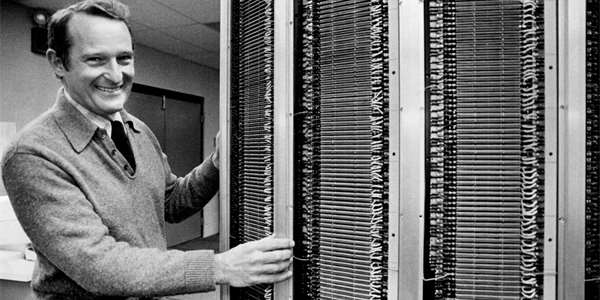
\includegraphics[width=0.5\textwidth]{Figures/seymour-cray.jpg}
	\caption{Seymour Cray \cite{Tronner20150626}}
	\label{fig:seymour-cray}
\end{figure}

Společnost Cray Research využívala ke konstrukci jejich superpočítačů až 10× rychlejší procesory v porovnání s procesory využívanými pro komerční počítače této doby. Později počátkem 90. let se však do popředí dostávají společnosti IBM a HP, které výkonem jejich superpočítačů zastiňují všechny menší firmy pokoušející se o vývoj vlastních superpočítačů.

V minulosti byly superpočítače navrhovány pro přesně danou úlohu. Příkladem takto specializovaného výpočetního clusteru je superpočítač Deep Blue, byl vyvinut společností IBM. Jeho úkolem bylo počítat postavení šachových figur na hracím poli. Tento superpočítač měl k dispozici 64 procesorů, na každou buňku hracího pole jeden. Deep Blue byl schopen spočítat až 200 milionů postavení šachových figur za sekundu. V květnu roku 1997 tento superpočítač porazil ruského šachového velmistra Garri Kasparova \cite{Hosch20191128}.

\begin{figure}[h]
	\centering
	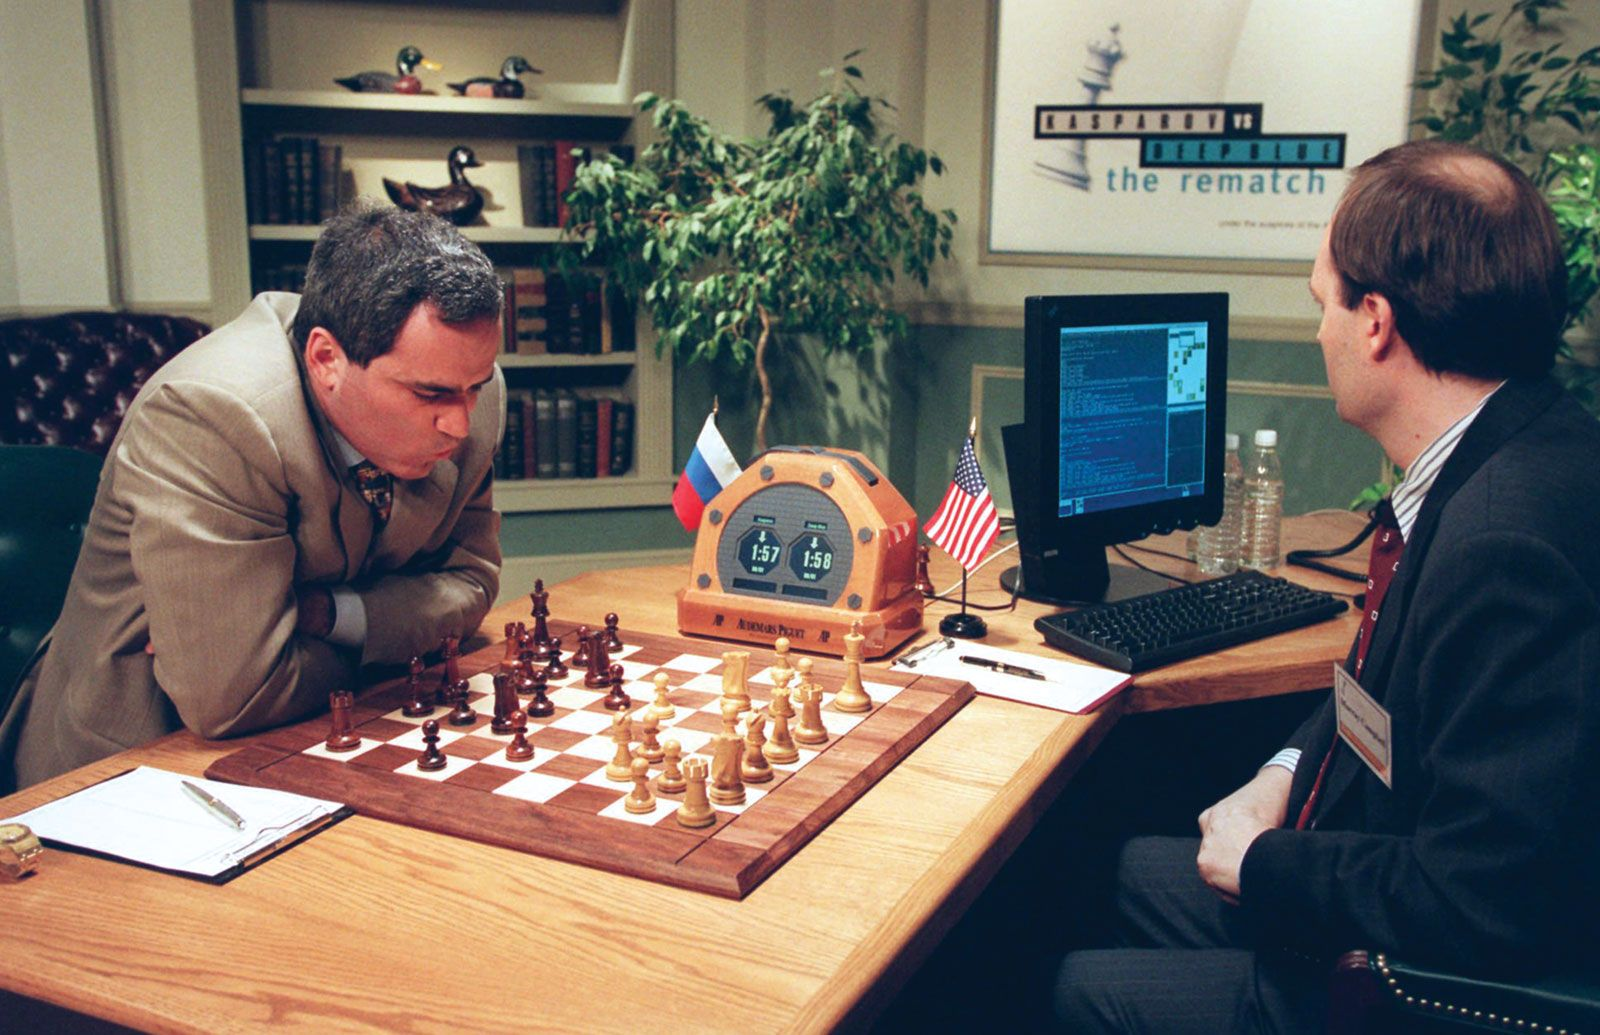
\includegraphics[width=0.5\textwidth]{Figures/Garry-Kasparov-playing-against-Deep-Blue.jpeg}
	\caption{Garry Kasparov hraje proti Deep Blue \cite{Hosch20191128}}
	\label{fig:garry-kasparov}
\end{figure}

\section{Výkon superpočítače}
Celosvětově využívanou metrikou pro měření výkonu superpočítačů je jednotka Flop/s. Jedná se o metriku, která je založena na počtu vykonaných operací v pohyblivé řadové čárce za sekundu. V době psaní této práce nejlepší superpočítače světa dosahují výkonu přes 440 PFlop/s.

Dle světového žebříčku TOP500 je nejvýkonnějším superpočítačem je v této době 
„Supercomputer Fugaku“ s ověřeným praktickým výkonem 442010 TFlop/s. Teoretický výkon tohoto clusteru je pak přes 537 PFlop/s, je počítán z udávaných hodnot frekvence použitých procesorů. Tento superpočítač má k dispozici přes 7,5 milionu jader a vlastní jej největší japonská vědecká instituce RIKEN \cite{B2TvJy8L3mSIxfWp}.

Nejvýkonnějším superpočítačem v České republice je nyní cluster Karolina s celkovým teoretickým výkonem 3,8 PFlop/s \cite{oviOzaWRPKlKSq7K}. Tento výpočetní cluster je umístěn v národním superpočítačovém centru IT4Innovations při Vysoké škole báňské – Technické univerzitě Ostrava. Superpočítač Karolina je v době psaní této práce umístěn na 71. pozici ve světovém žebříčku TOP500 \cite{iqgLoV1cXM0Qb6t1}.

Vývoj v odvětví IT se však žene stále kupředu a je jen otázkou času, kdy se v žebříčku objeví nový superpočítač a celé pořadí zpřehází.

\section{Plánovač úloh}
Výpočetní cluster je z praktického hlediska implementací dávkového systému. Uživatelé sami jejich programy na systému nespouští, ale dávají pokyn plánovači, který zajistí zpracování úlohy \cite{W94NKRaxvG2L2A1W}. Jedná se o program, který spravuje životní cyklus úloh na clusteru. Dle vypočtené priority řadí vytvářené úlohy do fronty, ze které jsou následně úlohy spouštěny. Stěžejními atributy pro zařazení úlohy do fronty mohou být například žádosti o množství zdrojů, doba zpracování nebo priorita úlohy.

Aby nedocházelo k plýtvání nevyužívaných zdrojů, tak je také jedním z hlavních faktorů zařazení úlohy do fronty využití samotných uzlů na výpočetním clusteru. Pokud tedy plánovač volí pořadí spouštění jednotlivých úloh, mezi metriky zařazuje i vlastní volné zdroje na kterých mohou být spouštěny kratší úlohy, i když pokyn k jejich zpracování přišel později než u časově náročnějších úloh.

I přes vysoký výkon superpočítačů a jejich neustálý vývoj není aktuálně možné uspokojit veškeré uživatelské požadavky ke zpracování úloh. Vytížení superpočítače a jeho zdrojů se průměrně pohybuje mezi 80-90 \%, každou dokončenou úlohu tak většinou nahrazuje úloha další. Uživatel tedy zpravidla na spuštění úlohy čeká. I tento problém pomáhá řešit plánovač na superpočítačovém clusteru. 

Následující obrázek \ref{fig:planovani-uloh} ilustruje plánování úloh s ohledem na co možná nejefektivnější využití výpočetních zdrojů. V tomto případě se jedná o dávkový systém se 6 výpočetními uzly. Cílem plánovače je zvolit pořadí spouštění úloh, tak, aby bylo minimalizováno plýtvání zdroji. Jednou z podmínek plánovače je omezení naplánování nanejvýš jedné úlohy na jeden uzel v jednom čase. V tomto příkladu se plánuje 9 úloh.

\begin{figure}[h]
	\centering
	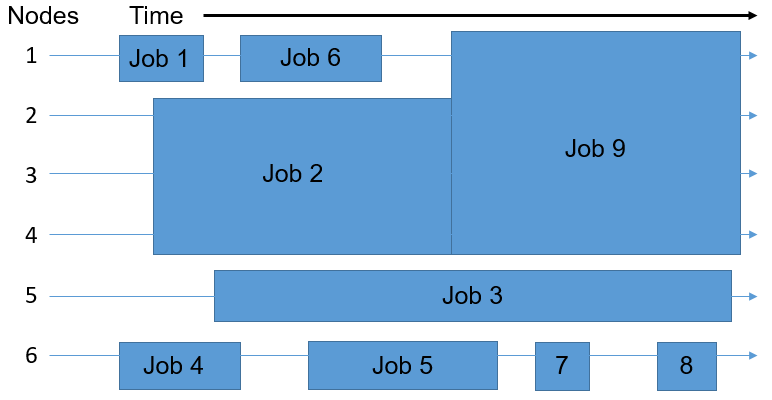
\includegraphics[width=0.7\textwidth]{Figures/Scheduler.png}
	\caption{Plánování úloh \cite{W94NKRaxvG2L2A1W}}
	\label{fig:planovani-uloh}
\end{figure}

Mezi hlavní úkoly každého plánovače se řadí zajištění spuštění každé úlohy (žádná úloha nesmí čekat ve frontě nekonečně dlouhou dobu), minimalizace nevyužití zdrojů a maximalizace průchodnosti úloh systémem.


\subsection{Plánovací algoritmy}
Jak už bylo popsáno výše, plánovač je odpovědný za řazení úloh do fronty. Další úlohou plánovače je přidělování zdrojů jednotlivým úlohám v době jejich běhu dle zásad a dostupnosti zdrojů. 

Mezi nejčastěji využívané plánovací algoritmy se řadí algoritmus zvaný FCFS (first-come first-served), tento algoritmus řadí úlohy do fronty dle časové posloupnosti jejich „příchodu do systému“. Tato fronta je pak v praxi označována jako fronta typu FIFO (first-in-first-out). 

K plánování HPC úloh může být také využit algoritmus ALCF (Argonne Leadership Computing Facility), princip tohoto algoritmu je obdobný jako u již zmiňovaného FCFS s rozdílem prioritizace časově náročnějších úloh a úloh, které jsou ve frontě již dlouhou dobu. 

Nejčastěji je však při plánování úloh využíváno techniky Backfilling. Technika Backfilling je optimalizovanou variantou algoritmu či principu FCFS, plánovač zkontroluje, zda je možné spustit první úlohu ve frontě. Pokud je to možné (je dostatek prostředků), úloha se spustí bez dalšího čekání. Pokud to však možné není, plánovač projde zbytek fronty a provádí kontrolu zda je možné spustit další úlohu, aniž by se prodloužila čekací doba první úlohy ve frontě \cite{pr00bfp79qnvRTQ3}.

Na obrázku \ref{fig:fcfs-without-backfilling} je ilustrována průchodnost systémem s využitím plánovacího algoritmu FCFS bez využití techniky Backfilling. Ilustrace \ref{fig:fcfs-with-backfilling} znázorňuje taktéž algoritmus FCFS s využitím techniky Backfilling. Při porovnání těchto ilustračních obrázků je možné vidět značné omezení plýtvání zdroji a maximalizaci průchodnosti systémem při použití techniky Backfilling. Bloky s čísly znázorňují plánované úlohy z fronty. Již běžící úlohy jsou označeny jako „running job“.
\newpage
\begin{figure}
	\centering
	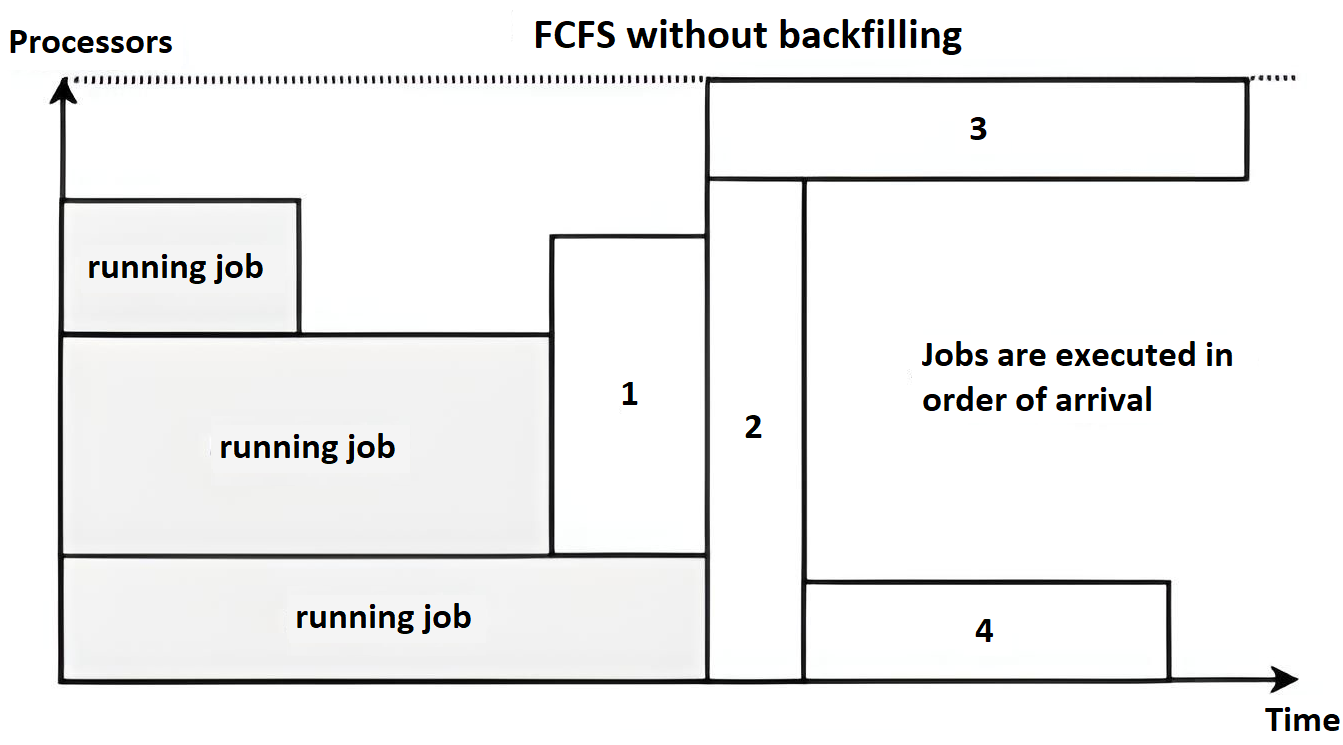
\includegraphics[width=0.8\textwidth]{Figures/fcfs-wb.png}
	\caption{Algoritmus FCFS bez použití techniky Backfilling \cite{GomezMartin2016}}
	\label{fig:fcfs-without-backfilling}
\end{figure}

\begin{figure}
	\centering
	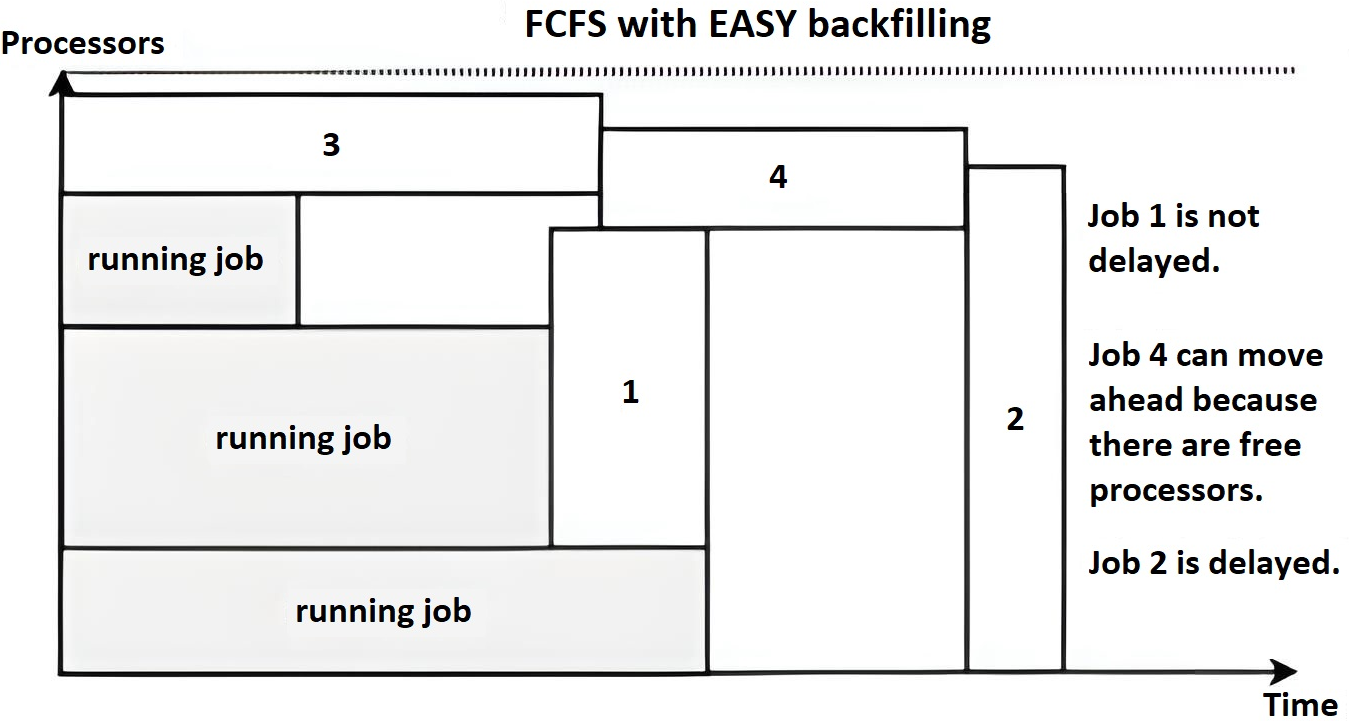
\includegraphics[width=0.8\textwidth]{Figures/fcfs-web.png}
	\caption{Algoritmus FCFS s použitím techniky Backfilling \cite{GomezMartin2016}}
	\label{fig:fcfs-with-backfilling}
\end{figure}

\chapter{State of the Art v oblasti HPC-as-a-Service}
Superpočítače a jejich výkon byl v minulosti vyhrazen pouze pro oblast výzkumu a vývoje. HPC bylo k dispozici vládním, lékařským, výzkumným organizacím a inovativním filmařům. K majoritním případům užití superpočítačů v této době patřily simulace jaderných testů, mapování lidského genomu nebo oživování dinosaurů ve filmech.

V současné době však dochází k masivnímu vzestupu datově náročných technologií. Typickým příkladem může být problematika umělé inteligence nebo problémy vyžadující masivní paralelismus\footnote{Masivní paralelismus je technika využívající velkého počtu procesorů či samotných počítačů k paralelnímu zpracování úloh.}. Tento fakt nutí širší okruh organizací zkoumat problematiku vysoce výkonného počítání. Ne každá společnost však má čas, peníze a odborné znalosti potřebné k jejich nasazení.

Z toho důvodu mohou tyto společnosti namísto náročného sestavování a správ superpočítačových clusterů využít již hotová řešení HPC jako služby (HPC-as-a-Service/HaaS). Díky HPC poskytovanému jako služba mohou organizace v některých případech spolupracovat s dodavatelem na konfiguraci infrastruktury, kterou potřebují pro své konkrétní výpočetní potřeby. Namísto nákupu nebo pronájmu hardwaru či softwaru si je však předplatí prostřednictvím modelu spotřeby „pay-as-you-go“.\cite{Rand20201203}

\section{Výhody HPC-as-a-Service}
HPC poskytované jako služba má výhody oproti hostování vlastní HPC infrastruktury. První důležitou výhodou může být model spotřeby „pay-as-you-go“, který byl již zmiňován výše. Zákazník tak platí jen za zdroje, které skutečně využil. Vlastní řešení, konstrukce a následná správa vysoce výkonných výpočetních clusterů je velmi náročná na zdroje.

Společnosti či organizace poskytující HPC-as-a-Service mají tendenci rychleji integrovat novější technologie. Tyto technologie jsou pak přístupné uživatelům využívající jejich služeb. Někteří poskytovatelé HaaS umožňují jejich zákazníkům provádění aktualizací či škálování\footnote{Škálování je pojem vyjadřující navyšování kapacit.} výpočetních kapacit na vyžádání. \cite{Wiggers20220120}

\section{Případy užití}
V dnešní době se poskytovatelé HPC-as-a-Service snaží co nejvíce přizpůsobit požadavkům jejich zákazníků. HaaS využívají společnosti, které pro řešení jejich problémů většinou vyžadují vysoký výkonného paralelní zpracování dat. Poměrně velký segment zákazníků tvoří oblast Automotive\footnote{Segment automobilového průmyslu.}, ti využívají HPC například ke zkrácení času simulací proudění tekutin či plynů. Při využití výpočetních clusterů nejen oboru Automotive dochází přesnějším a rychleji dosaženým výsledkům při vývoji. Dalším oborem, ve kterém je HPC hojně využíváno je obor lékařství, vývoj léčiv je díky masivnímu paralelnímu zpracovaní efektivnější a rychlejší, dochází pak i k minimalizaci vzniku chyb.

HPC je využíváno v mnoha dalších oborech či odvětvích, patří tam i obor výzkumu a vývoje. HPC umožňuje analyzovat rozsáhlé datové soubory v poměrně krátkém čase a sdílet výsledky se spolupracovníky. Dále je HPC využíváno třeba ke 3D modelování a renderování scén, toho využívají grafická,herní a filmová studia.

Obrázek \ref{fig:haas} ilustruje využití HPC-as-a-Service / HaaS.

\begin{figure}[!h]
	\centering
	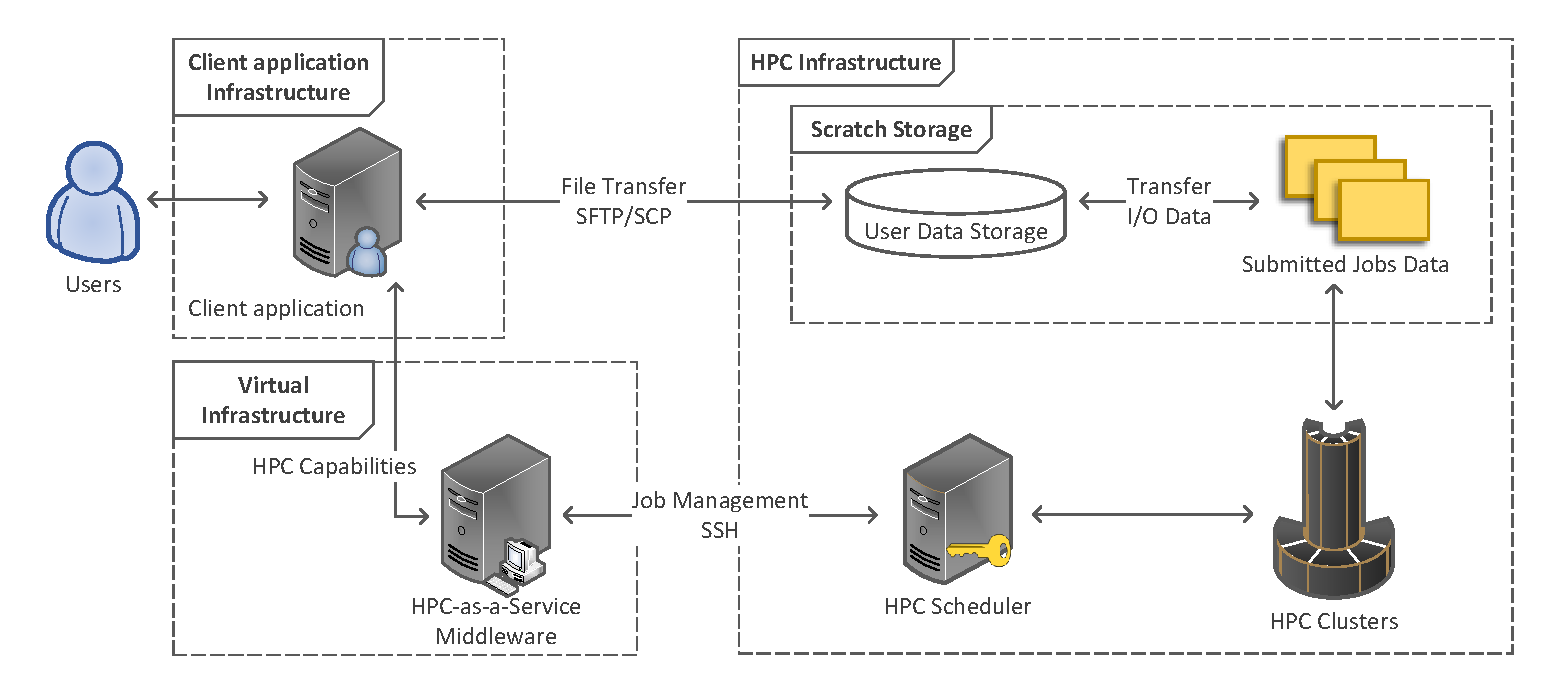
\includegraphics[width=1\textwidth]{Figures/haas.pdf}
	\caption{HPC-as-a-Service / HaaS \cite{uG7wIvjQiIli6kO9}}
	\label{fig:haas}
\end{figure}
\chapter{Seznámení s HEAppE Middleware}\label{chapter:chapter-about-heappe-middleware}
Kapitola je zaměřena na popis aplikačního rámce HEAppE Middleware.

\section{Účel HEAppE Middleware}
HEAppE Middleware (High-End Application Execution Middleware) poskytuje aplikační rozhraní (API) pro kompletní správu úlohy na superpočítačovém clusteru, od vytvoření až po přenos zpracovaných dat. Jedná se o Open-Source\footnote{Kód, který je navržen tak, aby byl veřejně přístupný.} projekt implementující koncept HPC-as-a-Service a jeho cílem je zjednodušit komunikaci s HPC plánovačem a umožnit uživateli pohodlnou implementaci do jeho klientské aplikace či systému. HEAppE Middleware zajišťuje bezpečnou a šifrovanou komunikaci s výpočetním clusterem prostřednictvím protokolu SSH. Komunikace pak stojí na autentizaci pomocí asymetrického šifrování s využitím veřejného klíče (RSA).

Abstraktně si můžeme HEAppE Middleware představit jako spolehlivého prostředníka mezi uživatelem a výpočetním clusterem, popř. jeho plánovačem. Poskytuje uživatelům vzdálený přístup k výpočetním clusterům se zaměřením na bezpečnost a jednoduchost přístupu.

Prakticky se jedná o službu, prostřednictvím které může koncový uživatel komunikovat s HPC clusterem přes standardizované aplikační rozhraní zvané jako REST API, stojící na HTTP komunikaci.

Následující obrázek \ref{fig:haas} ilustruje využití HPC-as-a-Service / HaaS.

\begin{figure}
	\centering
	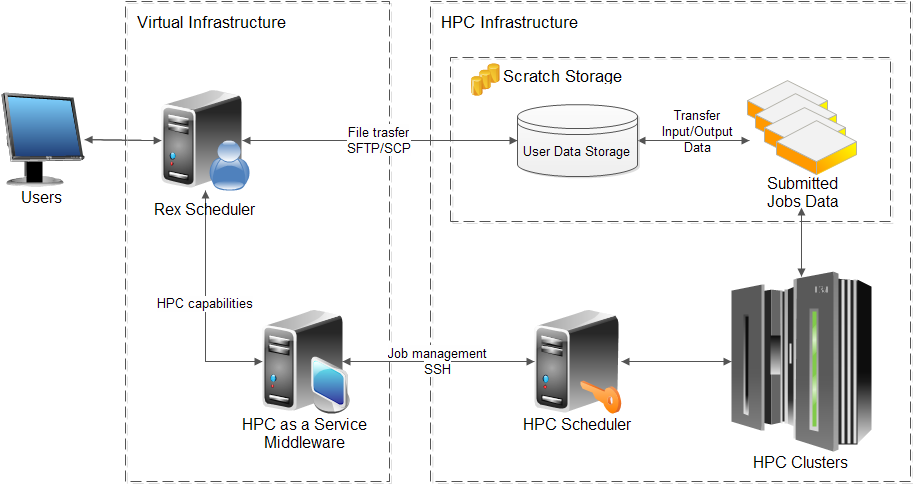
\includegraphics[width=0.8\textwidth]{Figures/haas.png}
	\caption{HPC-as-a-Service / HaaS \cite{uG7wIvjQiIli6kO9}}
	\label{fig:haas}
\end{figure}

\newpage
\section{Technické zázemí HEAppE Middleware}
Velký důraz je v tomto projektu kladen na multiplatformní využití a nezávislost použitého hardwaru. Tento aplikační framework je postaven na technologii .NET Core, poskytuje REST API a při nasazování je využívána kontejnerizační technologie Docker. Komunikace s plánovačem výpočetního uzlu probíhá prostřednictvím protokolu SSH, uživatel je autentizován jedním z uložených servisních účtů metodou RSA.

V současnosti tento framework zajišťuje komunikaci s plánovači PBS a Slurm. Podporuje autentizaci prostřednictvím SSH Agenta a je zajištěna podpora OpenID and OpenStack autentizace pro přístup k HEAppE Middleware API.

\subsection{Konfigurace HEAppE Middleware}
HEAppE je nutné před spuštěním konfigurovat. V první řadě je sestaveno konfigurační schéma (docker-compose) pro službu Docker, na které middleware běží. Do této konfigurace jsou zaneseny mimo obraz HEAppE Middleware všechny podpůrné služby, jako je MS SQL Server nebo SSH Agent. V návaznosti je přidána konfigurace samotné aplikace (AppConfig), která primárně specifikuje spojení s databází, port middleware API a další. Nedílnou součástí konfigurace je i počáteční stav dat uložených v databázi (seed), který si každý uživatel může specifikovat. Tato data jsou v okamžiku prvního spuštění HEAppE nahrána do databáze.

\subsection{REST API}
REST API je standardizované aplikační rozhraní využívající protokol HTTP. Služba poskytující toto API vystavuje tzv. endpointy (koncový uzel zpřístupněný uživateli) a specifikaci pro práci s nimi. V případě HEAppE Middleware se jedná o url adresy se specifikací JSON\footnote{JSON neboli JavaScript Object Notation je formát využívaný pro výměnu dat. Formát je jednoduše čitelný i pro člověka.\cite{lJoeVuQg92zsjaAe}} struktury dat, které systém na vstupu očekává. Z praktického hlediska může jít např. o komunikační bod pro vytvoření specifikace úlohy, na vstupu se očekává JSON struktura popisující úlohu a specifický řetězec, který uživatel obdrží po autentizaci na jiném endpointu.

\subsection{Protokol SSH a metoda šifrování RSA}
Jak už bylo popsáno výše, HEAppE Middleware ke komunikaci s HPC clustery využívá protokolu SSH. Koncový uživatel je od této komunikace odstíněn a komunikuje pouze s vrstvou REST API. Při navazování spojení SSH je také odesílán soukromý klíč jednoho z nastavených servisních účtů v HEAppE Middleware, ten je následně porovnán s veřejným klíčem uloženým na HPC clusteru. Tato komunikace uživateli zaručuje bezpečnost pro práci, hlavní výhodou asymetrického RSA šifrování je vysoká složitost pro dešifrování, metoda je založena na prvočíselném rozkladu a je v současné chvíli prakticky neprolomitelná.

Bezpečnost RSA je postavena na předpokladu, že rozložit velké číslo na součin prvočísel (faktorizace) je velmi obtížná úloha. Z čísla \emph{n = pq} je tedy v rozumném čase prakticky nemožné zjistit činitele \emph{p} a \emph{q}, neboť není znám žádný algoritmus faktorizace, který by pracoval v polynomiálním čase vůči velikosti binárního zápisu čísla n. Naproti tomu násobení dvou velkých čísel je elementární úloha.\cite{GqNaOav5DExhzgW6}

\subsection{Kontejnerizace a Docker}
Při nasazování HEAppE je využívána technologie Docker. Ta umožňuje nakonfigurovat systém a pak už jen HEAppE Middleware sestavit na libovolném serveru. Docker umožňuje uzavřít a spustit aplikaci v izolovaném prostředí zvaném kontejner, to umožňuje na hostitelském systému spustit několik kontejnerů současně. Kontejnery jsou oddělené a obsahují vše potřebné pro běh aplikace, takže se uživatel nemusí spoléhat na to, co je na hostitelském počítači aktuálně nainstalováno \cite{Ued4tuEOQL0cOIeN}. Docker automaticky stáhne požadované obrazy (image) a spustí aplikaci. 

Výhoda tkví především v přenositelnosti specifikace na jiné servery, kontejner je pak oddělen od ostatních, je možné specificky nastavit jeho komunikační rozhraní dle potřeb uživatele.

Architektura technologie Docker je ilustována na obrázku \ref{fig:docker-architecture}.

\begin{figure}
	\centering
	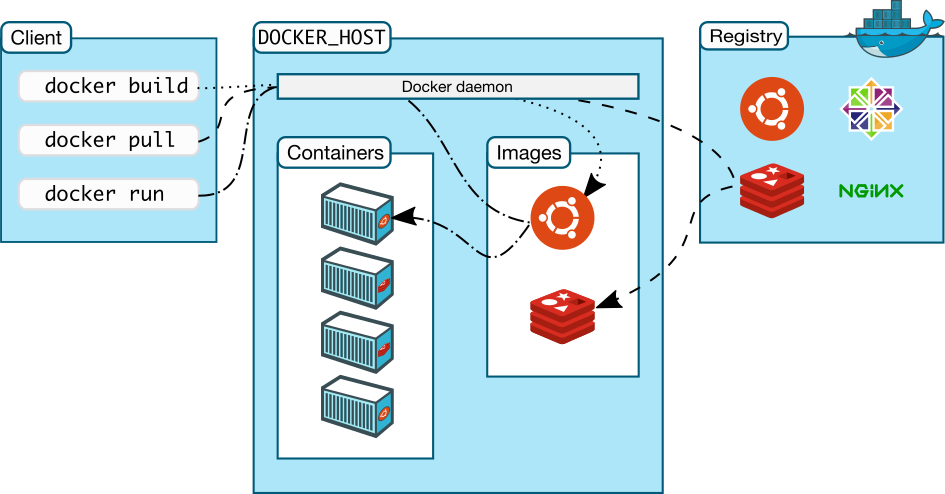
\includegraphics[width=0.8\textwidth]{Figures/docker-architecture.png}
	\caption{Archtektura Docker \cite{Ued4tuEOQL0cOIeN}}
	\label{fig:docker-architecture}
\end{figure}

\subsection{Plánovače PBS a Slurm}
HEAppE Middleware v době psaní této práce podporuje plánovače PBS a Slurm, tyto plánovače jsou hojně využívány v superpočítačových centrech po celém světě. Jedním z cílů HEAppE Middleware je platformí nezávislost, komunikační rozhraní jednotlivých plánovačů je však rozdílné a musí se k nim přistupovat individuálně. Koncový uživatel je však od této skutečnosti odstíněn a může tedy pracovat stále stejně, bez nutnosti znalosti dalšího systému. Na pozadí to řeší samotný middleware.


\section{Abstrakce HPC úlohy}
HEAppE Middleware poskytuje uživateli určitou míru abstrakce nad skutečnou specifikací HPC úlohy. Úloha je v HEAppE nazvána jako Task. Několik těchto Tasků tvoří Job, ten obsahuje obecné informace a nastavení, příkladem může být maximální doba běhu úlohy, zvolený cluster, maximální doba čekání na spuštění úlohy, definice proměnných využívaných při běhu programu. Každý z takto specifikovaných Jobů obsahuje minimálně jednu úlohu (Task), tedy samostatnou specifikaci spouštěné úlohy na clusteru. Těchto Tasků je možné definovat více, může u nich být specifikovaná i závislost na ostatní úlohy. Specifikace Tasku především obsahuje požadavky na využití jader, časový limit pro zpracování úlohy, frontu úloh a další specifické parametry pro běh spouštěného programu.

Tasky je možné spouštět jen z předem vytvořených šablon, ve kterých je definováno, jaký program se má na clusteru spouštět nebo jaké argumenty jsou u programu dostupné. Argumenty programu musí uživatel uvést vždy u specifikace úlohy (tasku).

Prostřednictvím HEAppE Middleware si uživatel definuje Job s Tasky, tento Job pak může spustit a kontrolovat jeho stav. V průběhu zpracovávání je možné kdykoli úlohu zrušit. HEAppE uživateli poskytuje možnost kompletně úlohu spravovat, a to bez nutnosti znalosti principů komunikace s plánovačem HPC clusteru.

Následuje příklad struktury příkazu ke spuštění úlohy na HPC clusteru, který plně nahrazuje jeden HEAppE RestAPI endpoint.

\begin{lstlisting}[language=bash,caption={Struktura příkazu qsub \cite{iR8VZfeCCZ757gs1}}]
qsub -q <queue> -w e -N <job_name> -l h_vmem=<memory> -l h_rt=<time> -l s_rt=<time> -pe smp <num_slots> -o <outputlogfile> -e <errorlogfile> <pathtoScript> <arg1> <arg2>
\end{lstlisting}

\section{Uživatelské a servisní účty}
HEAppE Middleware mapuje HEAppE uživatelské účty na skutečné clusterové účty (servisní). Správce HEAppE instance je oprávněn k vytváření uživatelských účtů. Uživatel se autentizuje prostřednictvím svého loginu a hesla, OpenID nebo OpenStack v HEAppE. Následně obdrží vygenerovaný klíč (alfanumerický hash) označovaný jako Session ID s časově omezenou platností. Při volání dalších HEAppE RestAPI endpointů tento hash využívá. Při konečné komunikaci se superpočítačovým clusterem HEAppE využívá jeden z uložených servisních účtů. Tyto účty jsou schváleny superpočítačovým centrem a správce HEAppE instance stojí za „nezávadností“ spouštěných úloh. 

HEAppE Middleware tyto clusterové (servisní) účty střídá, aby např. nedošlo k zablokování ze strany superpočítačového centra. Systém bez rotace využívaných servisních účtů by mohl nést znaky DOS/DDOS\footnote{DOS nebo také DDOS je typ útoku na internetové služby nebo stránky, jehož cílem je cílovou službu znefunkčnit a znepřístupnit ostatním uživatelům; může k tomu dojít zahlcením obrovským množstvím požadavků, ve variantně DDOS jde o distribuovaný DOS \cite{UUBpn6UTaV8mOipc}} útoku a účty by mohly být preventivně zablokovány.

Z výše uvedeného textu je zřejmé, že uživatelé spouštějící úlohy prostřednictvím HEAppE Middleware mohou ve skutečnosti využívat jeden servisní clusterový účet. HEAppE řeší přístupy uživatelů k jejich datům na výpočetním clusteru. Každý uživatel HEAppE se pak nemusí verifikovat přímo superpočítačovému centru, k použití stačí mít HAppE uživateslký účet.

\section{Zajímavé funkcionality HEAppE Middleware}
\subsection{JobArrays}
K úlohám definovaným prostřednictvím HEAppE je možné přidat specifikaci pro opakování spouštění úlohy. Tato funkcionalita je nazvána jako JobArrays, teminologie vychází z funkce plánovače. Uživatel specifikuje iterace dané úlohy a plánovač pak úlohu spouští v cyklu. Praktické využití této funkce je například u renderování scén a vykreslování grafiky.
Příklad formátu pro definování JobArrays:


\begin{lstlisting}[language=bash,caption={Struktura definice JobArrays}]
                            <start_index>-<end_index>:<step>
\end{lstlisting}

\subsection{Závislosti úloh}
U jednotlivých úloh je možné specifikovat jejich závislosti na jiných úlohách. Uživatel může jednoduše definovat závislosti úloh. Prakticky se jedná o podmíněné spouštění dalších navázaných úloh až po úspěšném vykonání úlohy předešlé. Omezuje se tímto možné plýtvání prostředky a výpočetním časem, které by mohlo nastat při selhání jedné z úloh, na jejímž výstupu závisí úloha další.

HEAppE ale musí řešit kontrolu těchto závislostí, aby plánovači byly zasílány validní specifikace úloh. Na straně výpočetního clusteru také probíhá kontrola specifikací, aby nedošlo ke kruhové/cirkulární závislosti. Zjednodušeně je tento problém možné specifikovat jako problém s nekonečným čekáním. Na straně výpočetního clusteru by mohl nastat tzv. Deadlock. Jedná se o uváznutí systému při vzájemném čekání. Na superpočítači se tento problém řeší kontrolou specifikace úloh a také detekcí kruhové závislosti v grafu. HEAppE cirkulární závislost kontroluje také, aby se celý proces urychlil a nedocházelo by k chybám na straně výpočetního clusteru. Na obrázku \ref{fig:cirkularni-zavislost} se nachází znázornění typického uváznutí – cirkulární závislosti procesů (P1, P2) a prostředků (R1, R2). Závislost je znázorněna šipkou.


\begin{figure}[!h]
	\centering
	
\includegraphics[width=0.6\textwidth]{Figures/Process_deadlock.png}
	\caption{Cirkulární závislost \cite{OvBwjLleECKerU0E}}
	\label{fig:cirkularni-zavislost}
\end{figure}

\newpage
\subsection{Extrémně dlouhé úlohy}
Každý uzel superpočítačového clusteru má definován horní interval pro dobu vykonávání uživatelských úloh, v praxi je tento časový parametr nazýván jako Walltime Limit. Systém ukončí každou úlohu, pokud přesáhne časový limit pro vykonávání úlohy. Existují ale uživatelé, jejichž programy vyžadují extrémně dlouhý čas pro dokončení, který překračuje již zmíněný limit na uzlu superpočítačového clusteru. I na tento problém HEAppE Middleware pamatuje. Při definování úlohy je možné nastavit přepínač pro vykonávání v režimu „ExtraLong“. V tomto případě HEAppE logicky rozdělí úlohu na více podúloh se závislostmi na postupném zpracování. Rozdělení pobíhá podle uživatelem uvedeného časového limitu a limitu pro zpracovávání na požadovaném uzlu superpočítače. Výhodou je to, že je uživatel odstíněn od manuálního rozdělování úlohy na podúlohy. Dále je takto upravená specifikace úlohy předána plánovači na superpočítači a ten se již stará o vykonání úlohy.

\hfill \break
\begin{figure}[h]
	\centering
	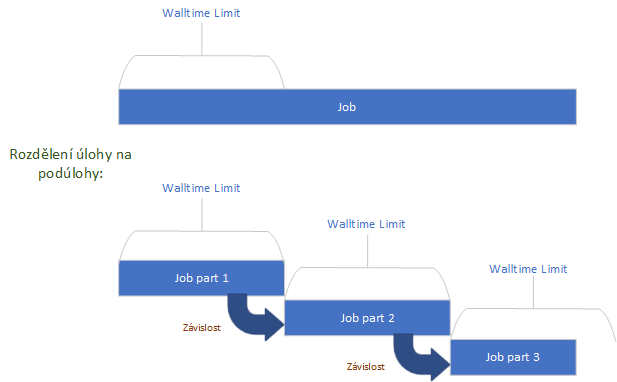
\includegraphics[width=0.8\textwidth]{Figures/job-decompose.png}
	\caption{Rozdělení extrémně dlouhé úlohy }
	\label{fig:rozdeleni-extra-long}
\end{figure}
\chapter{Rozšíření HEAppE pro lokální výpočty}
Jedním z hlavních cílů této práce je navrhnout a implementovat rozšíření HEAppE Middleware o možnost lokálních výpočtů, tedy umožnit uživateli nasimulovat spouštění úloh lokálně počítači s využití rozhraní HEAppE, a to bez nutnosti spojení se superpočítačem. Výhodou tohoto rozšíření je především možnost nezávislé přípravy specifikace úlohy a vyzkoušení práce s HEAppE.

Jelikož je systém HEAppE Middleware zpravidla nasazován za pomocí technologie Docker na servery superpočítačového centra, tak je možné tento způsob pohodlně replikovat i na uživatelském počítači. Technologie Docker je možné nainstalovat jako službu na počítače s operačními systémy MS Windows, macOS i Linux.

Cílem tohoto rozšíření je co možná největší udržení systémové nezávislosti. Mělo by simulovat HEAppE komunikaci s výpočetním clusterem. Na straně simulovaného HPC clusteru v prostředí uživatelského počítače by mělo být dosaženo co nejpodobnější chování plánovače, jako je tomu na skutečných výpočetních clusterech.

\section{Návrh řešení}
Toto rozšíření bylo navrženo s ohledem na platformní nezávislost a využití stávajících principů, na kterých stojí HEAppE Middleware.

Jelikož je HEAppE postaven na kontejnerizační technologii Docker, tak bylo navrženo, aby samotný virtuální HPC cluster byl spouštěn také jako kontejner. Pro uživatele by mělo být poměrně jednoduché řešení, neboť by šlo jen o malou úpravu stávající Docker konfigurace (přidání vazby na kontejner) a přidání záznamu virtuálního clusteru do databáze (popř. upravení tzv. seedu) – přesně tak, jak je tomu i při přidávání specifikace skutečného HPC clusteru.

Kompletní specifikaci kontejneru pro Docker i konfiguraci HEAppE databáze je možné sdílet s uživateli, kteří o lokální spouštění úloh mají zájem. Pro tyto uživatele by mělo být velmi jednoduché systém HEAppE s dodanými konfiguračními soubory sestavit, spustit a používat. 

Celá koncepce návrhu rozšíření se nachází na obrázku \ref{fig:navrh-rozsireni-o-lokalni-hpc-clsuter}.

\newpage
\begin{figure}
	\centering
	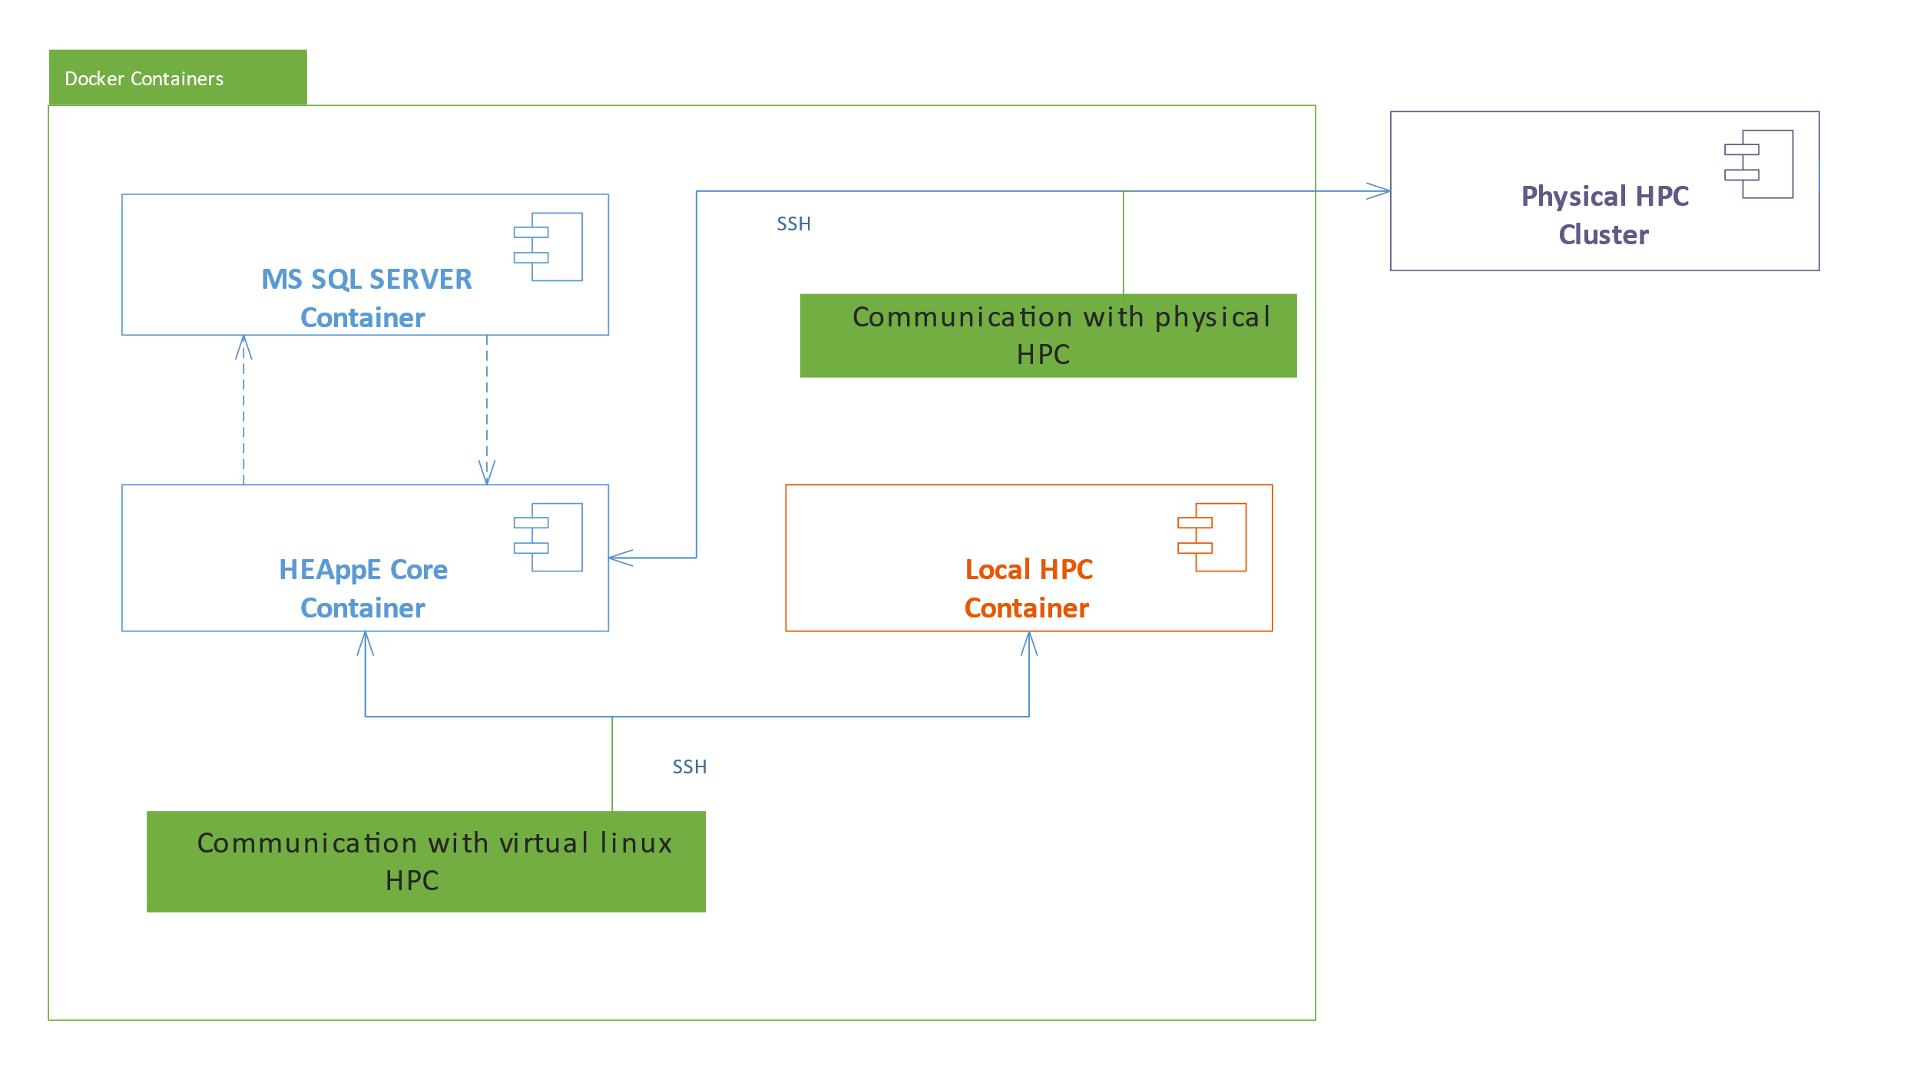
\includegraphics[width=1.0\textwidth]{Figures/local-hpc-clsuter-navrh.png}
	\caption{Návrh rozšíření o lokální HPC cluster}
	\label{fig:navrh-rozsireni-o-lokalni-hpc-clsuter}
\end{figure}

Lokální HPC Cluster je z technického hlediska instance virtuálního stroje s OS Linux. K nasimulování chování plánovače, který je součástí superpočítače, bude v tomto případě využito několik skriptů, které se budou spouštěny na žádost HEAppE. HEAppE Middleware bude upraven především ve vrstvě pro komunikaci s HPC plánovači, úpravy nebudou zasahovat do logiky užívání při spojení s plánovači na skutečných superpočítačích, a to i z důvodu možnosti zanesení chyby do stávajícího řešení. Aplikační rámec HEAppE Middleware bude rozšířen o konektor (SchedulerAdapter) pro práci s lokálním virtuálním strojem simulující chování plánovače na superpočítači.

Vrstvy v HEAppE jsou tvořeny s ohledem na pozdější úpravy či přidávání dalších adaptérů apod. Je využíváno návrhového vzoru Abstract Factory (abstraktní továrna), k tomuto návrhovému vzoru bude přihlíženo při výše popsaných úpravách.

\section{Konfigurace virtuálního stroje}
Nespornou výhodou použití Docker engine je snazší distribuce komponent systému. Pro jednotlivé kontejnery stačí vytvořit konfiguraci, popř. připravit obraz potřebných služeb. Služby v kontejneru jsou pak spouštěny dohromady, je mezi nimi možné vytvořit komunikační kanály. Právě tímto způsobem pak bude realizována komunikace mezi HEAppE a virtuálním HPC clusterem.

Výhodu je také to, že do konfigurace je možné zanést aktuální stav virtuálního stroje, tak aby koncový uživatel měl vše připraveno. V případě této instance budou nastaveny komunikační porty, vytvořen uživatel v systému OS Linux, uloženy skripty pro simulování komunikace s plánovačem, nebo zde např. budou připraveny testovací SSH-RSA klíče a povolena komunikace mezi kontejnery.

Tato konfigurace je v praxi označována jako dockerfile, jedná se o soupis kroků či povelů, které se stanou při spouštění kontejneru. Od stažení obrazu operačnío systému, až po zpřístupnění komunikačního portu.

Následuje ukázka využívaného dockerfile pro instanci lokálního HPC clusteru.

\hfill \break
\lstinputlisting[language=Dockerfile,caption={dockerfile konfigurace pro virtuální stroj},breaklines=true]{SourceCodes/dockerfile}

\section{Komunikace mezi HEAppE a virtuálním HPC}
Ke komunikaci mezi HEAppE a skutečným superpočítačovým clusterem probíhá především prostřednictvím protokolu SSH. Komunikace je založena na principu klient-server (heappe-HPC). Prostřednictvím SSH HEAppE odesílá příkazy např. pro vytvoření, spouštění úlohy apod. Zpět dostává od plánovače výsledek provedení příkazu či skriptu, vyžádaná data, popř. aktuální stav úlohy.

Obdobně byla navržena komunikace i mezi HEAppE a virtuálním strojem simulující chování plánovače superpočítačového clusteru. Komunikace taky probíhá prostřednictvím SSH s využitím autentizace, tak aby byla simulace co nejvěrohodnější.

\section{Data a stav úloh}
HEAppE Middleware je stavěn tak, že se na obou stranách (HEAppE i HPC) uchovávají data o prováděných úlohách. HEAppE si v době běhu úlohy na superpočítači cyklicky žádá o data. A postupně se takto obě databáze synchronizují. Dotazování na nová data končí v okamžiku ukončení úlohy. Data jsou poskytována pouze na vyžádání, nejedná se o sdílený datový prostor. Data jsou z HPC zasílána v předem známém formátu v textové podobě zpět při SSH komunikaci.

Obdobně je přistupováno k datům i v případě simulace HPC na lokálním virtuálním stroji. S ohledem na výkon a režii nejsou data na straně virtuálního HPC ukládána v databázi. V adresáři dané úlohy je sada souborů, obsahující data (stav, parametry) úlohy. Tato data se nachází v předem definované JSON struktuře, jsou ukládána a aktualizována při běhu úlohy. Po vyžádání jsou data zaslána v JSON struktuře textově zpět na HEAppE.

Pro práci s JSON strukturami slouží ve virtuálním stroji parser\footnote{Parser je program či jeho část provádějící syntaktickou analýzu textu. Analýza textu je proces, při němž je zpracováván text za pomoci definovaných pravidel daného jazyka.\cite{uEN4MdNhBpkZmkHF}} jq\cite{qibOqajDMnKYNjXq}. Jedná se o program, který je schopen spravovat JSOn struktury, umožňuje získat data nebo je aktualizovat či přidat a odebrat. Tento program je instalován při sestavování Docker kontejneru, žádost o instalaci se nachází v konfiguraci dockerfile.

\hfill \break
\begin{lstlisting}[caption={Příklad JSON struktury}]
{
   "SessionCode": "string",
   "CreatedJobInfoId": 0
}
\end{lstlisting}

\section{Implementace na straně HEAppE Middleware}
Jak už bylo zmíněno výše, HEAppE Middleware je stavěn na platformě .NET Core\footnote{.NET Core je Open-Source vývojová platforma sloužící k vytváření aplikací.}, vyvíjí se v jazyce C\#. Z hlediska pohledu architektury se jedná o vrstvený systém. Uživatelské požadavky na REST API jsou zachyceny ve stejnojmenné vrstvě (RestAPi). Z této vrstvy jsou vstupní data po úspěšné validaci předávána do servisní a BusinessLogic vrstvy, ve které se nachází primární aplikační logika. Na závěr se požadavek dostává do vrstvy HpcConnectionFramework.

Vrstva HpcConnectionFramework je místem, kde dochází ke komunikaci s výpočetními clustery. V této vrstvě je implementováno několik adaptérů, které jsou schopny pracovat s odlišnými typy plánovačů na superpočítačích. Adaptéry jsou voleny na základě specifikace úloh, HEAppE předem musí mít v databázi informace o používaných clusterech a plánovačích. Právě v tomto místě se také nachází největší část implementace pro komunikaci s lokálním simulovaným výpočetním clusterem.

Samotná implementace výše popsaného řešení se skládá z adaptéru, ve kterém se nachází logika pro komunikaci s virtuálním strojem. V tomto místě jsou připravovány příkazy ke spouštění skriptů pro řízení úloh a zpracovávány odpovědi lokálního HPC. Důležitou součástí je také datový konvertor, jehož úkolem je mapovat získaná data z lokálního HPC v JSON formátu na objekty nebo jejich kolekce. S těmito objekty je pak dále v HEAppE pracováno již obvyklým způsobem, jako je tomu u komunikace se skutečnými HPC. Nedílnou součástí celého adaptéru jsou připravené DTO \footnote{Objekt pro přenos dat.} objekty, přesněji se jedná o objekty popisující stav prováděné úlohy. Při konstrukci těchto objektů byl užit návrhový vzor Composite.

DTO objekty s napamovanými daty jsou pak v nižších vrstvách využity pro aktualizaci stavu a časů jednotlivých spouštěných úloh.

\section{Implementace na straně virtuálního stroje}
Konfigurace již zmiňovaného virtuálního stroje s OS Linux je sepsána jako sekvence kroků pro spouštění v prostředí Docker. Součástí konfigurace je stažení obrazu OS Linux (Minideb) vytvoření uživatele pro práci, nastavení přístupových práv, nastavení domovského adresáře, instalace openssh serveru pro komunikaci nebo například instalace programu jq pro jednodušší práci s JSON strukturami.

Z důvodu možnosti jednoduché a rychlé úpravy byly pro řízení běhu simulovaného plánovače napsány scripty ve skriptovacím jazyce BASH. Zmíněné skripty programátor může jednoduše číst, orientovat se v nich, a protože se jedná o interpretovaný jazyk, tak se programy napsané v BASH spouštějí přímo bez nutnosti kompilace. Pro využití s Docker konfigurací tyto programy patří mezi nejlepší možné rychlé a jednoduché řešení. Celkově tato koncepce navazuje na stávající řídící skripty, které HEAppE využívá na skutečných výpočetních clusterech pro zjednodušení komunikace. Tyto skripty byly zvalidovány služnou, která je dostupná na adrese \emph{\href{https://www.shellcheck.net/}{shellcheck.net}}.

Mezi stávající využívané skripty patří například skript vytvářející pracovní adresář pro dané úlohy, přidávání či odebírání SSH klíčů nebo skript pro přesun dat. Tyto stávající skripty jsou využívány i na skutečných výpočetních clusterech.

Parametry jednotlivých skriptů, které jsou zasílány z HEAppE jsou enkódovány do formátu Base64, aby nedocházelo k nechtěným problémům v případě zasílaných nepovolených znaků. Na straně virtuálního i skutečného výpočetního clusteru jsou tyto parametry dekódovány a užívány v textové podobě dle zvolené logiky.



\hfill \break
\lstinputlisting[language={},identifierstyle=\color{black},caption={Příklad Base64 kódování}]{SourceCodes/base64-enc.txt}

Byla vytvořena pětice skriptů, jejichž úkolem je nasimulovat chování plánovače. Jedná o skript, který slouží k přípravě úlohy, spouští úlohu, získává aktuální stav úlohy, ukončuje úlohu nebo získává počet úloh na simulovaném clusteru. Všechny tyto podpůrné skripty pracují jen se soubory a adresáři, aby nedocházelo ke zbytečné zátěži hostitelského počítače (není použit DB server apod.). 

\subsection{Skript pro přípravu úlohy}
Tento skript po spuštění připraví specifikace a parametry úlohy do kořenového adresáře úlohy na simulovaném HPC clsuteru. JSON struktura s popisem úlohy je vložena do souboru \emph{.job\_info}. Příkazy kódované v Base64 jsou uloženy do souboru \emph{.commands}. S těmito soubory, přesněji s jejich obsahem pracující další skripty, které jsou popsány níže.


\subsection{Skript pro spouštění úlohy}
Skript věrohodně simuluje chování postupného spouštění jednotlivých úloh, ty se staví do fronty. Využívá program jq k úpravám JSON struktury celé úlohy, která je uložena v souboru adresáře úlohy. Skript pracuje následujícím způsobem:

\begin{enumerate}
	\item Načtení předaných parametrů pro spouštění (příkazy uložené v souboru \emph{.commands} v kořenovém adresáři dané úlohy)
	\item Rozdělení jobů na jednotlivé na sebe navazující tasky
	\item Zapsání aktuálního času do stavové struktury úlohy (soubor \emph{.job\_info} v kořenovém adresáři dané úlohy)
	\item Zapsání stavu R (running) a PID (process ID) do stavové struktury
	\item Správa jednotlivých tasků (s ohledem na jobArrays, závislosti)
	\begin{enumerate}
		\item Vstup do adresáře tasku
		\item Uložení dat do stavové struktury k danému tasku (stav, čas)
		\item Spuštění úlohy
		\item Uložení stavu a času po dokončení úlohy
	\end{enumerate}
	\item Vstup do adresáře jobu
	\item Zapsání stavu a časů daného jobu (agregace stavů úloh)
	\item Ukončení scriptu
\end{enumerate}

Aktualizace datové struktury pro ukládání stavů (v souboru \emph{.job\_info}) je okamžitě propsána do souboru po každé úpravě z důvodu nemožnosti předvídání čtení aktuálního stavu prostřednictvím HEAppE. Data musí být v každém kroku aktuální.

\subsection{Skript pro získání stavové struktury úlohy}
Po vyžádání dat (spuštění skriptu s parametry úlohy) je přistoupeno do adresáře úlohy a na výstup skriptu jsou odeslána data v textové podobě (JSON). Tato data jsou pak přijata v HEAppE a jak již bylo výše popsáno, jsou namapována na DTO objekty, se kterými se dále pracuje a v posledním kroku dojde k synchronizaci dat s databází HEAppE.

\subsection{Skript pro získání počtu úloh}
Skript na výstupu vrací počet adresářů s úlohami, které byly prostřednictvím HEAppE a řídících skriptů na straně simulovaného HPC clusteru vytvořeny. Tento skript je využíván pro získávání informací o clusteru pomocí HEAppE endpointu. Výstupem je report s jednoduchou statistikou užívání daného clusteru.

\subsection{Skript pro ukončení aktuálně běžící úlohy}
Protože HEAppE podporuje ukončení aktuálně běžící úlohy na HPC clusteru, tak bylo nutné vytvořit skript i pro virtuální HPC cluster, který ukončí právě běžící proces, jenž je reprezentací úlohy či agregací úloh. Tento skript přečte uložené číslo procesu (PID) na lokálním stroji simulující chování HPC plánovače, které se nachází v souboru \emph{.job\_info} a vyšle zprávu danému běžícímu procesu (příkaz kill). Následně jsou změněny stavy a časová razítka ve struktuře úlohy na virtuálním HPC clsuteru.

\section{Nutné kroky ke spuštění}
V případě, že chce uživatel využívat HEAppE s rozšířením pro simulaci výpočtu na lokálním počítači, tak musí provést následující kroky.

\begin{enumerate}
	\item Získání konfigurace kontejneru pro simulaci HPC se všemi skripty a soubory (obsahuje konfiguraci dockerfile)
	\item Úprava docker konfigurace HEAppE pro spouštění kontejnetu lokálního clusteru (příklad níže)
	\item Přidání clusteru do výchozího stavu dat databáze (seed)
	\begin{enumerate}
	    \item Protože se bude jednat o kumunikaci mezi Docker kontainery, musí být atribut MasterNodeName, který se využívá jako Host při nastavování spojení na cluster, nastaven na hodnotu "host.docker.internal" – není možné využít adresu localhost ani 127.0.0.1
	    \item Musí být nastaveny údaje pro autentizaci (username, password, private key, key file)
	    \item Musí být vytvořen nový uzel s frontou, kterou uživatel bude využívat na virtuálním HPC
	    \item Atribut SchedulerType musí být nastaven na hodnotu 1, interně je v logice HEAppE tento typ plánovače využit při volbě adaptéru ve vrstvě HpcConnectionFramework
	\end{enumerate}
\end{enumerate}

\begin{lstlisting}[language=Dockerfile,caption={Docker konfigurace pro spouštění kontejnetu lokálního clusteru}]
localhpc:
    container_name: localhpc
    build: C:/path/to/LocalLinuxHPCclusterConf
    ports:
    - "49005:22"
\end{lstlisting}


Popis nutného nastavení s přesnými údaji je uveden v textovém souboru u samotné konfigurace kontejneru.

Bod č. 1 je možné nahradit za spuštění Docker kontejneru lokálního clusteru zvlášť. Bez návaznosti na ostatní služby HEAppE.


V příloze se nacházejí přesnější ukázky výše popsaných segmentů, které je nutné přidat do konfigurace dat pro databázi HEAppE (seed).






\chapter{Uživatelsky definované šablony výpočtů}
Dalším cílem této práce je navrhnou a implementovat řešení, které uživateli umožní jednoduchou správu šablon výpočtů (vytváření, modifikace a mazání). Taková šablona (v HEAppE nazvaná jako Command Template) obsahuje cestu k programu na clusteru a požadované parametry daného programu. Uživateli bude zpřístupněn nový endpoint na REST API, pomocí které bude možné novou šablonu vytvořit.

V současné chvíli HEAppE poskytuje funkcionalitu pro vytvoření tzv. generického command template, prakticky se jedná o dynamicky se vytvářející šablonu za běhu. Generická šablona bude použita pro vývoj tohoto řešení.

\section{Generická šablona}
Generic command template je postaven tak, že není nutné měnit jeho specifikaci při změně spouštěné aplikace na superpočítačovém clusteru. Uživatel tedy může používat generickou šablonu a spouštět různé typy výpočtů. Při vytváření úlohy se využije místo klasického Command Template tato generická šablona. Tato šablona se využívá primárně pro účely testování, pro pravidelné užívání je určena přesně definovaná šablona, která je uložena v databázi HEAppE. Ta obsahuje cestu ke skriptu, který je spouštěn při vykonávání úlohy a set požadovaných argumentů skriptu.

Generická šablona obsahuje parametry, ve kterých uživatel specifikuje cestu ke skriptu, který chce spustit a ve speciálním formátu zadá také parametry. Na clusteru se nachází skript, který spustí zadaný skript s parametry zadané uživatelem.

Před samotným spuštěním se však provádí validace zadaných parametrů a existence skriptu na clusteru. Skript, který je spouštěn prostřednictvím generické šablony výpočtů musí obsahovat hlavičku s parametry skriptu. Tato hlavička je v HEAppE přečtena a následně jsou názvy předaných argumentů či parametrů porovnány se zadanými parametry uživatelem.

\newpage
\begin{lstlisting}[language=bash,caption={Ukázková hlavička skriptu s „generickými" parametry iterations a message}]
#!/bin/bash
#HEAPPE_PARAM iterations
#HEAPPE_PARAM message
\end{lstlisting}

Po validaci je na clusteru spuštěn řídící skript, který namapuje zadané parametry na proměnné, které je následně možné v programu využít.

\section{Návrh řešení}
Aby si uživatel mohl před přesnou specifikací nově vytvářené šablony výpočtů šablonu vyzkoušet, bude uživatelské vytváření nových šablon výpočtů navázáno na generickou šablonu výpočtů. Při vytváření nové šablony uživatel uvede stejné údaje, jako při užívání generické šablony ve specifikaci úlohy.

Během vytváření šablony výpočtů bude zkontrolován uživatelem zadaný skript (hlavička s parametry) pro požadované názvy parametrů. Pokud bude vše souhlasit, šablona výpočtů se vytvoří.

Další funkcionalitou bude modifikace již existující šablony výpočtů, editovat bude možné atributy, které jsou ke specifikaci tzv. Commmand Template využívány. Pokud uživatel změní cestu k cílovému skriptu, který se spouští na clusteru, tak dojde i ke změně dostupných parametrů skriptu. Tyto parametry musí být uvedeny v hlavičce cílového skriptu. V čase změny musí být již tento skript dostupný na superpočítačovém clusteru.

Součástí správy šablon výpočtů je i mazání existujících Command Template. Tato funkcionalita však nebude fyzicky mazat záznamy daných Command Template z databáze z důvodu možných referencí na úlohy. Pokud by v databázi existiovala šablona výpočtů, která již byla použita ve specifikaci HPC úlohy, tak by bylo nutné kaskádově smazat záznamy ze všech tabulek, které obsahují referenci na Command Template. Tato funkce tedy bude nastavovat příznak IsEnabled na False v daném záznamu Command Template. To ale není možné, když tento příznak bude nastaven na False, tak jej systém HEAppE neumožní dále využívat. Bude třeba upravit logiku aplikace, upravit model a vytvořit novou migraci databáze\footnote{Migrace databáze je proces při které dochází k verzování databáze/modelu aplikace.}.  

Výše popsané funkcionality budou dostupné jako endpointy na REST API HEAppE Middleware. Bude vytvořen nový Management controller\footnote{Controller je část systému HEAppE reagující na události přicházející od uživatele.} v kódu HEAppE. Pro využívání těchto funkcionalit bude oprávněn pouze uživatel s rolí Administrátora.

\section{Implementace}
Do vrstvy REST API byl přidán nový controller a trojice endpointů s názvem CreateCommandTemplate, EditCommandTemplate a RemoveCommandTemplate, pro mapování dat zadaných uživatelem byly vytvořeny třídy popisující vstupní data. Dále byla upravena servisní vrstva a vrstva aplikační (business) logiky, tak aby bylo možné implementovat výše popsané funkcionality HEAppE. 

Po obdržení žádosti na endpointu CreateCommandTemplate proběhne validace, zda zadaná generická šablona existuje a zda-li odkazovaný skript obsahuje v hlavičce názvů parametrů, přesněji se jedná o přečtení hlavičky skriptu. Hlavička má z definice jednoznačný formát, proto se při parsování názvů parametrů z textu využívá regulárního výrazu.


\begin{lstlisting}[language=bash, caption={Regurální výraz pro parsování názvů parametrů}]
                                #HEAPPE_PARAM ([A-z0-9]+)\n
\end{lstlisting}

Po úspěšné kontrole je vytvořen objekt CommandTemplate s vazbou na skript a parametry. Následně je šablona uložena do databáze a připravena k použití.

Správa šablon je složitější operace, předpokládá se, že správu jednotlivých šablon bude provádět poučená osoba pro práci s HEAppE pro další uživatele, kteří se starají primárně o vytváření a spouštění úloh. Proto je funkcionalita dostupná pouze pro uživatelé s rolí Administrátora.

Analogicky dle výše popsaného návrhu řešení fungují endpointy EditCommandTemplate a RemoveCommandTemplate.

\section{Prerekvizity pro správné fungování}
Předpokladem pro vytváření nových šablon výpočtů je existence generické šablony v systému HEAppE. Dále musí uživatel vytvořit skript, který bude chtít spouštět společně s hlavičkou obsahující parametry ve výše uvedeném formátu. Při vytváření uživatel také může uvést další parametry pro tvorbu šablony výpočtů.



\begin{lstlisting}[caption={JSON struktura pro endpoint CreateCommandTemplate}]
{
  "SessionCode": "string",
  "GenericCommandTemplateId": 0,
  "Name": "string",
  "Description": "string",
  "Code": "string",
  "ExecutableFile": "string",
  "PreparationScript": "string"
} 
\end{lstlisting}




\chapter{Testování softwaru}
Cílem testování softwaru je zjištění kvality daného softwaru, zda splňuje veškeré smluvené nároky například na výkonnost nebo správnost řešení a pomáhá odhalovat chyby. Testování je nedílnou součástí vývoje SW, obvykle se software či jeho části testují průběžně. A to především z důvodu včasného odhalení chyb, které je možné v průběhu vývoje snáze opravit. Testování softwaru může sloužit jako prostředek k mitigaci rizik, cílem je snížení či eliminace rizik spojených s nasazením chybného kódu do produkčního prostředí.

\section{Historie testování}
První chyba či selhání celého počítače bylo zaznamenáno v padesátých letech 20. století na Harvardově univerzitě. Chyba však nestála na straně softwaru, nýbrž příčinou byla zaklíněná můra v součástkách tehdejšího sálového počítače s označením Mark II, a ten vypověděl službu. Z tohoto prostého důvodu se dnes při řeči o chybách v programu využívá označení „moucha“ či „bug“. Prvotně toto označení použil Thomas Edison v jeho publikacích z 19. století, nyní však šlo o první počítačovou chybu. 

Chyba v programu vede k selhání softwaru. Záznam o této chybě vzniknul v roce 1945. Podařilo se dochovat i onu můru, tedy strůjce celého problému \cite{85SxcMZY6LKfV8v4}. Kopie tohoto záznamu se nachází na obrázku \ref{fig:zaznam-o-prvni-chybe}.


\begin{figure}[!h]
	\centering
	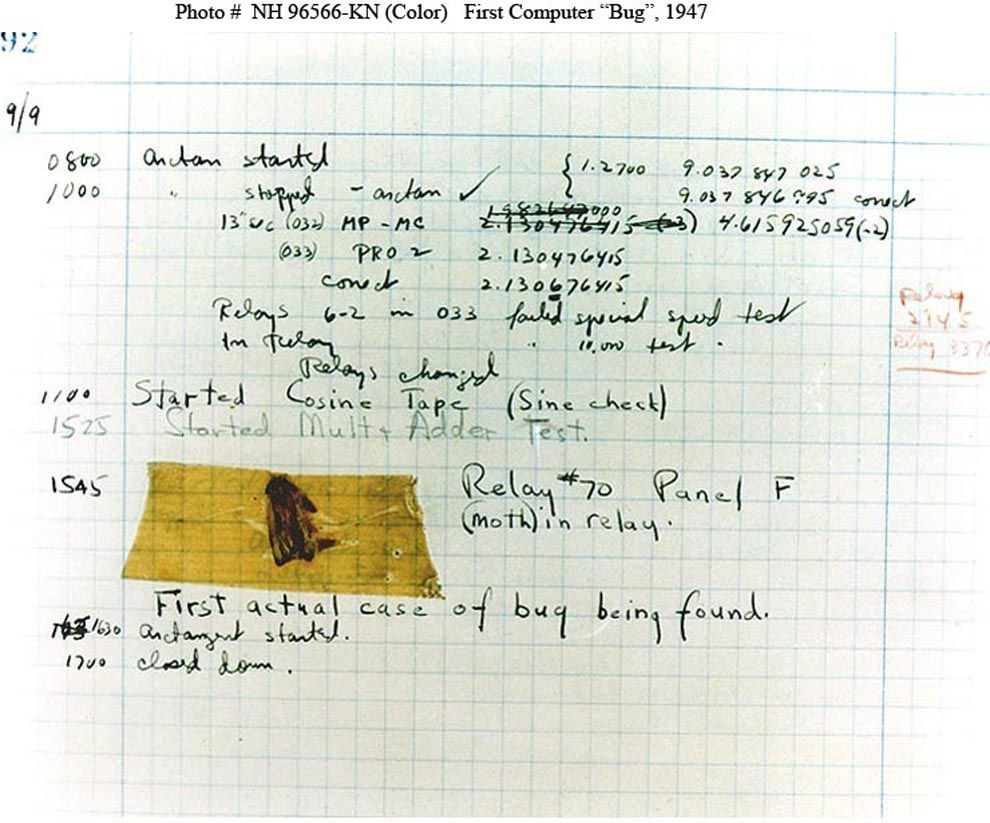
\includegraphics[width=0.5\textwidth]{Figures/first-pc-bug.jpg}
	\caption{Záznam o první počítačové chybě \cite{85SxcMZY6LKfV8v4}}
	\label{fig:zaznam-o-prvni-chybe}
\end{figure}

\section{Proces vývoje softwaru}
Mezi základní modely popisující proces vývoje softwaru patří model velkého třesku, model „programuj a opravuj“, vodopádový model nebo spirálový model. Mezi stěžejní body propracovanějších modelů se řadí specifikace, vývoj a testování. Každý tým vyvíjející software si může tento proces definovat tak, aby byl efektivní a splňoval očekávané podmínky zadavatele. Metodika či proces vývoje softwaru obvykle kombinuje hned několika principů z výše vyjmenovaných modelů. Především se však proces ubírá směrem iteračního vývoje softwaru. Vývoj softwaru v iteracích či cyklech vychází z praktických zkušeností především z důvodu přicházejících změn či doplňování specifikací už při vývoji softwaru.

Velmi důležitým krokem celého procesu vývoje softwaru je testování. Testování slouží především k odhalování chyb, které mohly být při vývoji zaneseny do kódu, a na první pohled nemusí být jasné, že se v kódu tyto chyby nacházejí. Proto je hned několik principů, jak software testovat. Metodiky testování se liší u různých projektů, a z praxe je zřejmé, že i přes sebelepší postup při testování softwaru je možné, že se chyba objeví až při užívání aplikace zákazníkem (obecně uživatelem). Cílem testování je minimalizace možnosti objevení chyb až ve fázi, kdy aplikaci využívá koncový uživatel. Některé testy či testové sady je možné automatizovat a zefektivnit tak fázi testování.

\subsection{Model velkého třesku}
Metoda vývoje, při které se využívá modelu velkého třesku stojí, na jednoduchosti celého konceptu. Veškeré úsilí je soustředěno na vývoj softwaru – konečného produktu. Model počítá s velmi nízkou úrovní specifikace výsledného softwaru. Součástí tohoto modelu není fáze formálního tetování \cite{Patton2002}. Model je vyobrazen na obrázku \ref{fig:big-bang-model}.


\begin{figure}[!h]
	\centering
	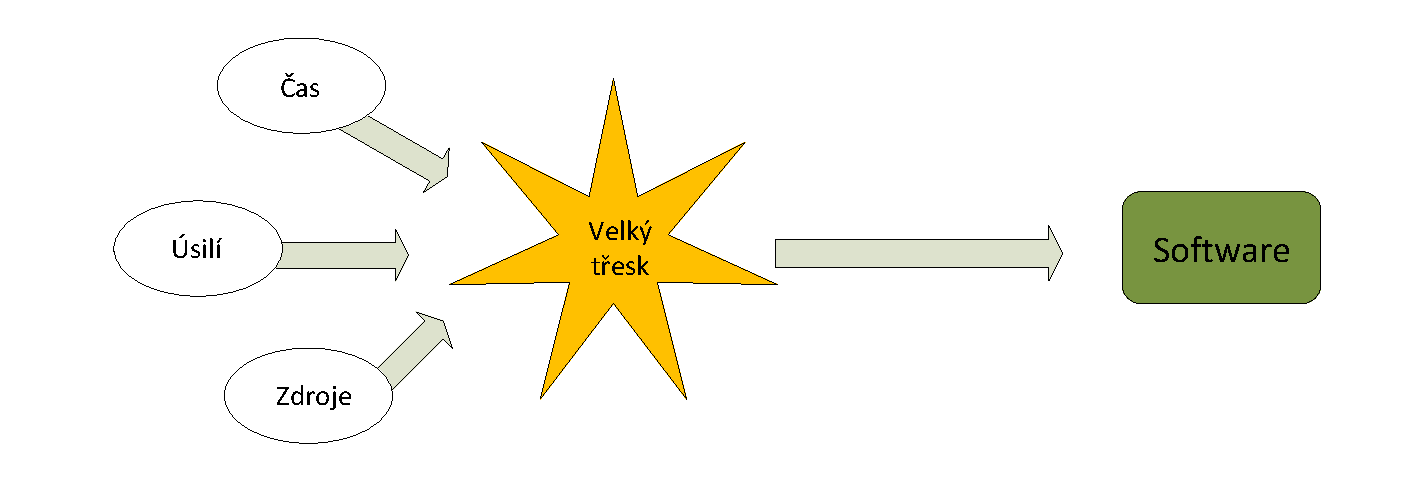
\includegraphics[width=0.8\textwidth]{Figures/VelkyTresk.pdf}
	\caption{Model velkého třesku}
	\label{fig:big-bang-model}
\end{figure}
\newpage
\subsection{Model „programuj a opravuj“}
Tento model nevyžaduje příliš mnoho režie či řízení. Je určen pro malé projekty vyžadující prezentaci výsledků v rychlém sledu. Začíná se hrubou představou o finálním softwaru, pokračuje cykly vývoje, testování a opravou chyb. Po několika iteracích těchto cyklů je rozhodnuto o ukončení práce \\a vydání softwaru. Model „programuj a opravuj“ se v praxi využívá např. u prototypů \cite{Patton2002}. Model je vyobrazen na obrázku \ref{fig:program-and-repair-model}.


\begin{figure}[h]
	\centering
	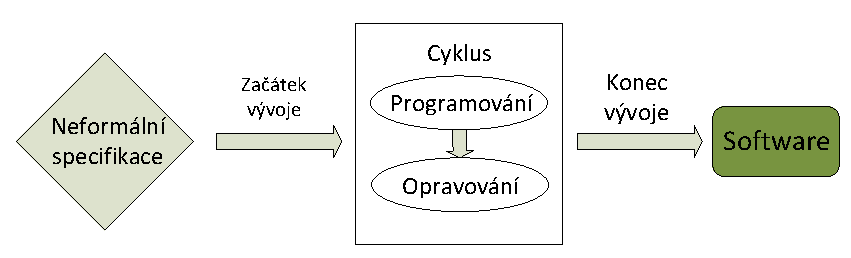
\includegraphics[width=0.8\textwidth]{Figures/ProgramujOpravuj.pdf}
	\caption{Model „programuj a opravuj“}
	\label{fig:program-and-repair-model}
\end{figure}

\subsection{Vodopádový model}
Vodopádový model spočívá v kontinuálním vývoji s přesně danou specifikací. Jednotlivé kroky tohoto modelu jsou atomické, nepřekrývají se a „není cesty zpět“. V jednotlivých krocích není možné postupovat zpětně, musí se dokončit daná iterace a začít specifikací znova \cite{Patton2002}. Model je vyobrazen na obrázku \ref{fig:waterfall-model}.

\begin{figure}[!h]
	\centering
	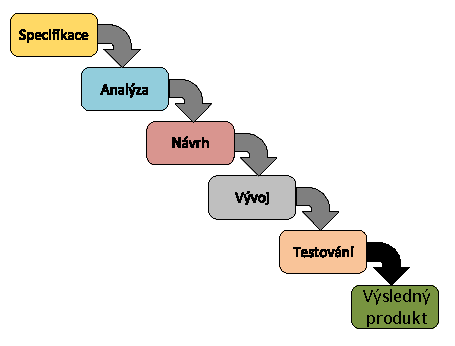
\includegraphics[width=0.5\textwidth]{Figures/waterfall.pdf}
	\caption{Vodopádový model}
	\label{fig:waterfall-model}
\end{figure}
\newpage

\subsection{Spirálový model}
Spirálový model řeší nedostatky výše uvedených modelů. Vývoj softwaru, který se řídí postupem daným spirálovým modelem je efektivní. Nevýhodou může být podstatně větší režie, než tomu bylo u modelů jako je model velkého třesku či model vodopádový. Jednotlivé kroky ve spirálovém modelu se mohou na rozdíl od vodopádového modelu překrývat \cite{Patton2002}.

V modelu jsou patrné 4 skupiny akcí, které je třeba provádět. Jmenovitě se jedná o plánování, analýzu rizik, vývoj a zhodnocení. Vývoj podle tohoto modelu probíhá v iteracích, při každém průchodu cyklem je pomyslně dokončena další část spirály. Model je vyobrazen na obrázku \ref{fig:spiral-model}.


\begin{figure}[!h]
	\centering
	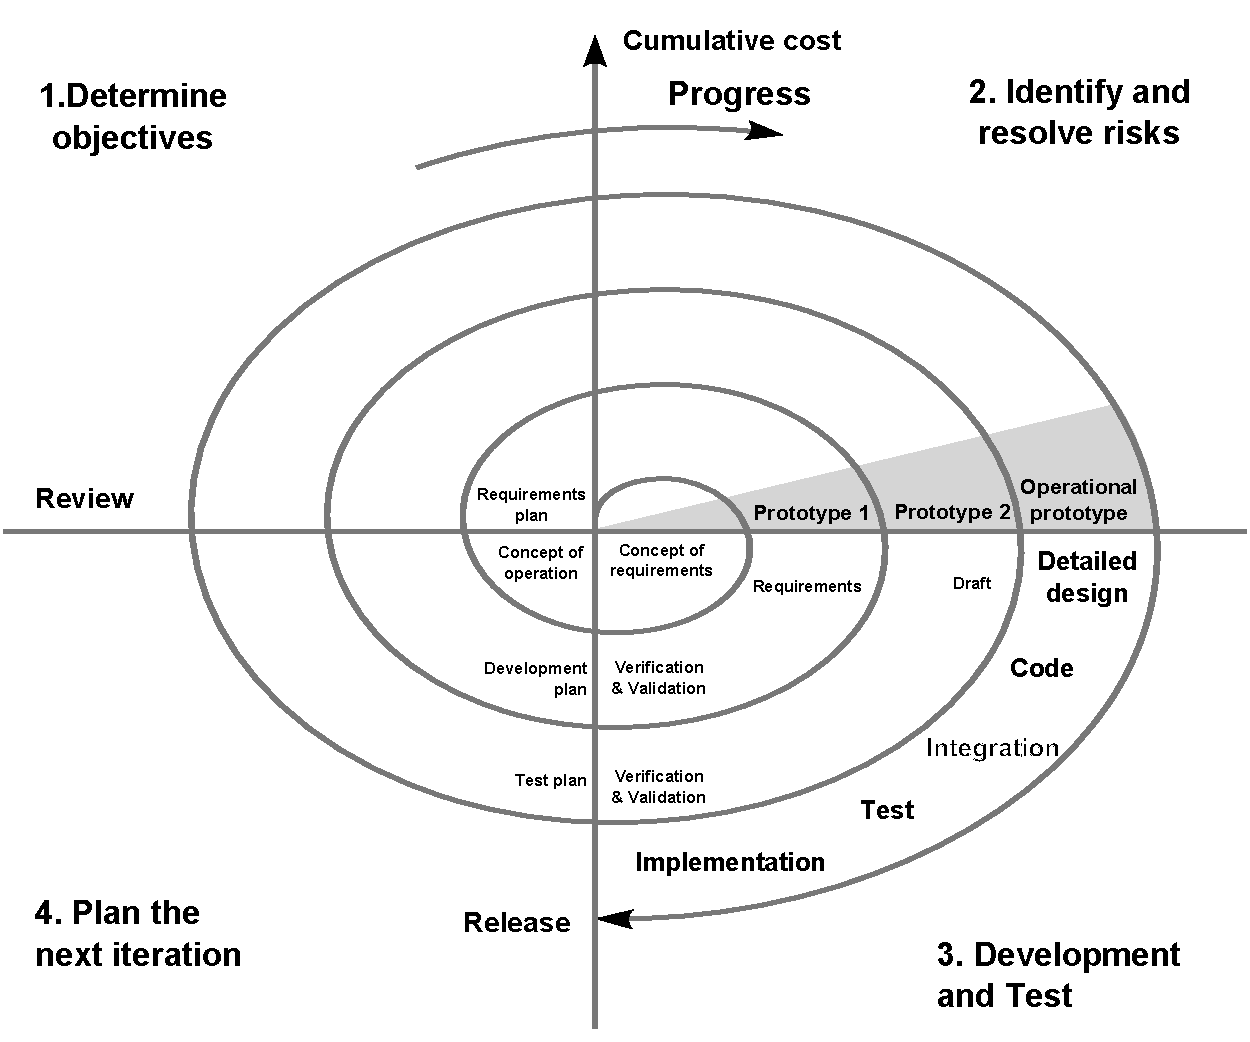
\includegraphics[width=0.58\textwidth]{Figures/Spiral_model.pdf}
	\caption{Spirálový model \cite{ee27bbyhk5LP1Ekm}}
	\label{fig:spiral-model}
\end{figure}

\newpage
\section{Testování API}
Předchůdcem API bylo vzdálené volání procedur (RPC), které vycházelo z potřeby zpracovávaní velkých dat či náročných komplexních výpočetních operací. V této době už k řešení zmíněných problémů nestačily procesory v osobních počítačích. Proto se zavedla metoda distribuovaných výpočtů, při kterých uživatelé výkon svých počítačů sdíleli. Možnost rozdělit úlohy na více částí se ale neobešla bez potíží. Například pokud někdo vypnul svůj počítač v době, kdy byl využíván ke vzdálenému zpracování úloh jiných uživatelů, mohlo dojít k tomu, že se proces vypnul, aniž by dokončil svou práci.

V dnešní době můžeme hovořit o dvou typech API. První možností je lokální aplikační rozhraní využívané například k interakci s operačními systémy nebo databázemi. Příkladem API operačního systému může být systémové volání pro čtení ze souboru. Tato systémová volání jsou programátorovi však skryta za funkcemi programovacích jazyků.

Z druhého pohledu na aplikační rozhraní se jedná o způsob propojení organizací či aplikací. Toto propojení může zajišťovat vzájemnou integraci. Strana využívající API tak nemusí implementovat své vlastní řešení, které již strana poskytující API vyřešila. Na straně druhé může dojít na straně poskytovatele API k chybě, v tomto případě může u strany využívající API dojít také k problémům, které je nutné řešit \cite{Mitchell2015}.


\section{Manuální a automatizované testování}
Testování softwaru je možné rozdělit do dvou základních skupin. Manuální testování zpravidla provádí člověk. Naopak automatizované testování zajišťuje stroj, který dle zvoleného scénáře většinou generuje požadavky na systém a čeká na odpověď, kterou porovnává s předpokládaným výstupem.

Automatizované testování nám může v krátkém čase přinést mnoho zajímavých výsledků. Dává nám náhled na to, na co se v daném systému zaměřit. Stojí však na poměrně náročném vytváření testových plánů či schémat. V případě nalezení chyby při automatickém testování se ale obvykle \\k problému musí dostat v posledním kroku i člověk, jehož úkolem je nalezení chyby v kódu. Využití automatizovaných testů je nesporně výhodné, především z časových důvodů, neboť můžeme stejné scénáře spouštět několikrát za sebou, např. s upravenými vstupy, které si můžeme nechat generovat. Výstupem automatizovaného testování je většinou souhrn či stručný přehled akcí, které se provedly. Tyto akce jsou pak označeny, zda se výstup rovná očekávanému výstupu. V případě projektu HEAppE Middleware jde o testování rozhraní REST API.

Automatizace testování je takřka nutností. Manuální techniky jednoduše neumožňují dostatečné testování ke zmírnění rizik, vzhledem k tomu, že jedno API samo o sobě může vyžadovat stovky testů, které je ve většině případů nutné opakovat \cite{Mitchell2015}.



\section{Framework pro automatizované testování HEAppE}
Mezi základní úkoly pro automatizované testování softwaru se řadí výběr frameworku\footnote{Framework je set programů, knihoven a rozhraní, které programátorovi zjednodušují práci. Framework většinou stačí nakonfigurovat a používat.}. Pro účely HEAppE Middleware byl vybrán Robot Framework \cite{UDdvJfGpGdOGQs2a}. Jedná se o automatizační Open-Source framework, který pracuje s vytvořenou provozuschopnou aplikací či API. Tento framework se využívá na úrovni integračního testování, v praxi jde o tzv. smoke testy \cite{K35ZsSqAfq3Ec1XJ}. Hlavním úkolem smoke testů je rychlé vyhodnocení funkčnosti aplikace, aby bylo možné přejít k dalšímu vývoji. Pomáhají odhalit nefunkční části aplikace či aplikačního rozhraní. Robot Framework je schopný pracovat \\s grafickým uživatelským rozhraním, ale pracuje i na úrovni REST API.

Robot Framework je nezávislý na operačním systému, jádro frameworku pak stojí na běhovém prostředí Python Interpreter\footnote{Python Interpreter převádí kód psaný v jazyce Python do jazyka strojových instrukcí, tyto instrukce jsou následně spouštěny a program v jazyce Python je vykonáván.}. To umožňuje především snadnou rozšiřitelnost a použitelnost. Základem automatizovaného testování prostřednictvím Robot Frameworku je sestavení testovacích plánů. Jedná se o popis akcí, které má framework vykonat. V případě HEAppE Midleware bude Robot Framework testovat endpointy REST API, pro dané požadavky pak budou dynamicky vytvářeny JSON specifikace. Základním plánem pro automatizované testování bude autentizace, vytvoření \\a spuštění úlohy. Tento plán může být dále rozšiřován.

Velkou výhodou tohoto frameworku je možné napojení na průběžnou integraci ve fázi vývoje. Průběžná integrace (Continuous Integration) slouží k urychlení nalezení chyb, integrace je spouštěna na integračním serveru podle předem zvoleného schématu. Metoda průběžné integrace je využívána i v projektu HEAppE, v průběhu sestavování aplikace je možné provést sadu testů z Robot Frameworku. Vývojáři pak budou mít lepší přehled o funkčnosti systému v dané fázi vývoje. Průběžná integrace je spouštěna předem nastavenou akcí. Může se například jednat o úpravu repositáře\footnote{Repositář je typ datové úložiště verzovacího systému.} či dané větve repositáře projektu. Sestavení a smoke testy jsou pak spouštěny automaticky, vývojář tak může sledovat stav integrace s informacemi o provedených testech. Metoda Continuous Integration je znázorněna na obrázku \ref{fig:ci}.

\begin{figure}[h]
	\centering
	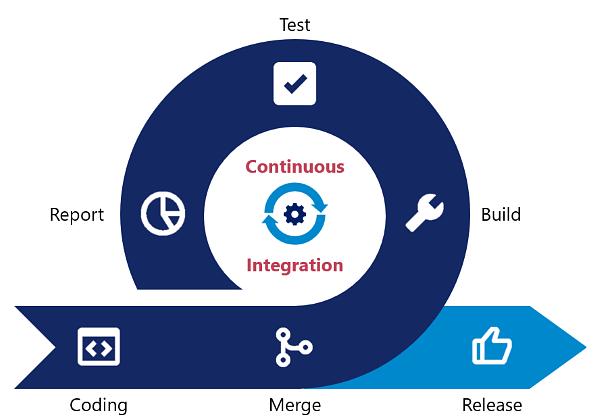
\includegraphics[width=0.6\textwidth]{Figures/cicd.png}
	\caption{Průběžná integrace \cite{cGNjWevJUlEHf7YF}}
	\label{fig:ci}
\end{figure}

\newpage
\section{Testovací scénář pro HEAppE}
Robot Framework je skvělým kandidátem pro testování hotových softwarových řešení. Pomocí tohoto frameworku je možné otestovat aplikační rozhraní daného systému z pohledu uživatele. Pro komplexní otestování HEAppE je možné vytvořit několik testovacích scénářů, které na sebe mohou navazovat. Základním scénářem pro používání HEAppE Middleware je vytvoření a spuštění úlohy na výpočetním clusteru. Z tohoto případu užití vychází i základní scénář pro automatizované testování HEAppE prostřednictvím Robot Framework.

Důležitým krokem při užívaní HEAppE Middleware je provedení autentizace. HEAppE po úspěšné autentizaci uživatele vrátí vygenerovaný unikátní identifikátor, který uživatel následně přidává do každé další žádosti při volání endpointu.

Hlavním úkolem tohoto testovacího plánu bude otestování spouštění úloh na výpočetních clusterech. Na každý cluster bude podána žádost o spuštění několika konfigurací úloh tak, aby byly otestovány všechny varianty specifikací úloh.

Součástí této práce je vytvoření testovacího plánu k otestování funkcionalit HEAppE při užívání rozšíření pro lokální spouštění úloh. Testovací plán taktéž bude testovat nově vytvořené endpointy v sekci Management, které jsou určené ke správě šablon výpočtů (Command Template).

\newpage
Před spouštěním úloh budou otestovány funkcionality související s uživatelem HEAppE. Tyto kroky se nachází v následující tabulce \ref{tab:user-testing}.

\begin{table}[!h]
	\centering
		\begin{tabular}{|C{0.8cm}|c|c|}
		    \hline
		    Krok & Název & Endpoint \\
		    \hline
			1 & Získání seznamu dostupných clusterů & \specialcell{/heappe/ClusterInformation/\\ListAvailableClusters}\\
			\hline
			2 & Autentizace uživatele & \specialcell{/heappe/UserAndLimitationManagement/\\
			AuthenticateUserPassword}\\
            \hline
			3 & \specialcell{Získání využití zdrojů a limity\\ uživatele HEAppE} & \specialcell{/heappe/\\UserAndLimitationManagement/\\GetCurrentUsageAndLimitationsForCurrentUser}\\
            \hline
            4 & \specialcell{Získání využití zdrojů na výpočetních \\clusterech} & 	\specialcell{/heappe/ClusterInformation/\\CurrentClusterNodeUsage}\\
            \hline
            5 & Získání využití zdrojů uživatele HEAppE & \specialcell{/heappe/JobReporting/\\GetUserResourceUsageReport}\\
            \hline
            6 & \specialcell{Získání využití zdrojů skupiny uživatelů\\HEAppE} & \specialcell{/heappe/JobReporting/\\GetUserGroupResourceUsageReport}\\
            \hline
		\end{tabular}
	\caption{Seznam kroků pro testování funkcionalit souvisejících s uživatelem HEAppE}
	\label{tab:user-testing}
\end{table}

Dále bude otestováno spouštění pěti různě specifikovaných úloh na superpočítačových clusterech s různými typy plánovačů. Kroky určené k otestování jedné úlohy popisují kroky uvedené v tabulce \ref{tab:task-testing}. 

Zmiňovaná pětice specifikací úloh obsahuje úlohy popsané v následujícím seznamu. Konfigurace těchto úloh byly popisovány výše v kapitole \ref{chapter:chapter-about-heappe-middleware}.

\begin{itemize}
    \item Základní úloha
    \item Úloha využívající generickou šablonu výpočtů
    \item Úloha se specifikací extrémně dlouhé úlohy
    \item Úloha využívající funkcionality JobArrays
    \item Úloha s definovanou závislostí na jiné úloze
\end{itemize}


\begin{table}[!h]
	\centering
		\begin{tabular}{|C{0.8cm}|C{6.9cm}|c|}
		    \hline
		    Krok & Název & Endpoint \\
		    \hline
			1 & Vytvoření úlohy & \specialcell{/heappe/JobManagement/CreateJob}\\
			\hline
			2 & Spuštění zpracování úlohy & \specialcell{/heappe/JobManagement/SubmitJob}\\
            \hline
			3 & \specialcell{Získání spotřebovaných zdrojů úlohy} & \specialcell{/heappe/JobReporting/\\GetResourceUsageReportForJob}\\
            \hline
            4 & \specialcell{Získání využití zdrojů na výpočetních \\clusterech} & 	\specialcell{/heappe/ClusterInformation/\\CurrentClusterNodeUsage}\\
            \hline
            5 & \specialcell{Získání stavu úlohy} & \specialcell{/heappe/JobManagement/GetCurrentInfoForJob}\\
            \hline
            6 & \specialcell{Vyčkání na spuštění úlohy} & \specialcell{/heappe/JobManagement/GetCurrentInfoForJob}\\
            \hline
            7 & \specialcell{Získání IP adres alokovaných uzlů} & \specialcell{/heappe/JobManagement/GetAllocatedNodesIPs}\\
            \hline
            8 & \specialcell{Zrušení úlohy} & \specialcell{/heappe/JobManagement/CancelJob}\\
            \hline
            9 & \specialcell{Vyčkání na ukončení úlohy} & \specialcell{/heappe/JobManagement/GetCurrentInfoForJob}\\
            \hline
            10 & \specialcell{Smazání úlohy} & \specialcell{/heappe/JobManagement/DeleteJob}\\
            \hline
		\end{tabular}
	\caption{Seznam kroků pro testování úloh HEAppE}
	\label{tab:task-testing}
\end{table}
\newpage

Provedením kroků, které se nacházejí v tabulce \ref{tab:task-testing-management}, se otestuje funkčnost již výše popsané správy Command Template. Implementace tohoto rozšíření HEAppE o správu Command Template je taktéž součástí této práce. Dle specifikace jsou Management endpointy dostupné jen uživateli HEAppE s rolí Administrátor.


\begin{table}[!h]
	\centering
		\begin{tabular}{|C{0.8cm}|C{6.9cm}|c|}
		    \hline
		    Krok & Název & Endpoint \\
		    \hline
			1 & Vytvoření Command Template & \specialcell{/heappe/Management/CreateCommandTemplate}\\
			\hline
			2 & Modifikace specifikace Command Template & \specialcell{/heappe/Management/ModifyCommandTemplate}\\
            \hline
			3 & \specialcell{Smazání Command Template} & \specialcell{/heappe/Management/\\RemoveCommandTemplate}\\
			\hline
		\end{tabular}
	\caption{Seznam kroků pro testování Management sekce HEAppE}
	\label{tab:task-testing-management}
\end{table}
\newpage

Protože je práce s úlohou na výpočetním clusteru řízena plánovačem, prakticky se jedná o předávání pokynů. Proto se v testovacím plánu musí vyskytovat čekání na vykonání příkazu. Při pokynu pro spuštění úlohy tak musíme čekat na to, až naši úlohu spustí plánovač na výpočetním clusteru. V testovacím scénáři je toto čekání implementováno opakovaným voláním HEAppE REST API s prodlevou, aby nedošlo k zablokování (toto chování by mohlo nést znaky DOS/DDOS útoku). Následuje ukázka kódu testovacího scénáře Robot Frameworku obsahujícího popsané cyklické volání REST API. V tomto případě se cyklus ukončí, pokud HEAppE vrátí stav, který značí, že je úloha spuštěna. Očekává se, že se stav změní v rámci jednotek či desítek minut, Robot Framework neumožňuje práci s cykly s neznámým počtem opakování. Proto byl při implementaci využit cyklus se známým počtem opakování, horní interval cyklu byl nastaven na maximální povolenou hodnotu.

Útržek testovacího scénáře obsahuje funkci WaitForJobRuns. Úkolem této funkce je počkat na spuštění úlohy plánovačem na výpočetním clusteru.


\lstinputlisting[language=bash, caption={Segment Robot Framework testu}]{SourceCodes/wait-for-job-runs.txt}

Výsledkem tohoto testování je vygenerovaný report a log. Programátor pak má lepší představu \\o funkčnosti jednotlivých částí systému. Tyto reporty Robot Framework připraví v grafické podobě. Dostupné jsou ve formátu html. Surová data jsou součástí reportu ve struktuře XML\footnote{Výměnný formát pro přenos dat}.




Test či testový plán může být prováděn pravidelně a několikrát za sebou. Počáteční časové náklady na sestavení tohoto scénáře jsou nesrovnatelné s přínosem, které automatizované testování přináší. Test navíc může běžet v pozadí automaticky a vývojář si tak jen vyzvedne výsledek.


Tento testovací scénář je možné volně rozšiřovat nebo vytvářet scénáře obdobné. Velmi praktické je i využití Robot Frameworku pro testování softwaru v době vývoje. Scénář můžeme měnit podle aktuálních požadavků např. při vývoji nové funkcionality.

Výše popsaný testový scénář byl použit k otestování funkčnosti HEAppE Middleware s užitím lokálního spouštění úloh na hostitelském počítači. Tímto byla prokázána validita implementovaných rozšíření, které popisuje tato práce. Pro uživatele je užití lokálního simulovaného clusteru prostřednictvím HEAppE takřka nerozeznatelné od použití HEAppE se skutečným výpočetním clusterem.

Navíc byly otestovány další endpointy, které je vhodnější testovat manuálně. Jedná se především \\o funkcionality HEAppE Middleware pro přenos dat, kdy je vhodnější provádět kontroly ručně.
Výsledky těchto automatizovaně prováděných testů jsou součástí práce v kapitole příloh v sekci \ref{chapter:robot-framework-local-tests}. 

Manuálně byly otestovány endpointy \emph{/heappe/FileTransfer/GetFileTransferMethod} a \emph{/heappe/FileTransfer/EndFileTransferMethod} za pomocí aplikace, která je součástí repositáře HEAppE. Tyto endpointy slouží k otevření přenosového kanálu mezi klientským počítačem a superpočítačovým clusterem. Funkcionalita tedy umožňuje přenos souborů mezi fyzickým počítačem uživatele \\a superpočítačovým clusterem. Při tomto testování byl otevřen přenosový kanál, pomocí protokolu SCP\footnote{Protokol sloužící k bezpečnému přenosu mezi dvěma počítači.} byl na cluster přesunut soubor, a následně byl přenosový kanál uzavřen. Výsledek tohoto testu se nachází v kapitole příloh v sekci \ref{manual-tests}.


\chapter{Závěr}
Při návrhu a implementaci podpory simulovaného plánovače spouštěného na lokálním stroji uživatele byla vytvořena konfigurace virtuálního stroje, jehož cílem je simulace chování superpočítačového clusteru s plánovačem úloh. Důraz byl kladen také na co možná nejvěrohodnější simulaci chování a komunikaci plánovače na lokálním virtuálním clusteru. Virtuální stroj byl navržen tak, aby jej uživatel mohl jednoduše upravit či zaměnit za své řešení. Musí přitom však dodržovat předepsané podmínky pro komunikaci HEAppE s lokálním simulovaným výpočetním clusterem.

Cílem tohoto rozšíření je přinést uživatelům možnost vyzkoušet si HEAppE Middleware na svém počítači bez nutnosti napojení na fyzický superpočítač. Proto je i komunikace s lokálním simulovaným výpočetním clusterem probíhá stejně, jako je tomu u skutečných výpočetních clusterů. Využívá se stejných protokolů, metod šifrování nebo postupů při autentizaci. To vše proto aby byl následný přechod z lokálně simulovaného prostředí na skutečné superpočítače co nejsnazší.

Dále bylo navrženo a implementováno rozšíření o funkcionalitu pro vytváření uživatelsky definovaných šablon. Prerekvizitou je existence generické šablony, která slouží především k testovacím účelům. Z této generické šablony se pak vychází při definování uživatelské šablony, která je následně uložena persistentně do systému HEAppE. A koncový uživatel ji může libovolně využívat.

Všechny nově přidané funkcionality byly důkladně otestovány, současný stav projektu s těmito změnami umožňuje publikaci do nové verze HEAppE Middleware. Současně byl vytvořen testovací scénář pro automatizované testování, který je možné spouštět při každé publikaci změny do repozitáře projektu.

Věřím, že díky výše popsaným funkcionalitám bude dále systém HEAppE Middleware rozšiřován do superpočítačových center, především díky rozšíření o možnost lokálního spouštění úloh. Uživatelé si budou moct HEAppE před nasazením v daném superpočítačovém centru vyzkoušet na svém počítači bez nutnosti přístupu na skutečné clustery. Jedním z účelů přidání této funkcionality je podpora popularizace HEAppE Middleware.
\endinput

% Seznam literatury
\printbibliography[title={Literatura}, heading=bibintoc]

% Prilohy
\appendix
\chapter{Příklad jednotlivých segmentů specifikace pro lokální HPC}
\lstinputlisting[caption={Sruktura segmentů konfigurace pro lokální HPC cluster}]{SourceCodes/add-specification.txt}
\chapter{Spuštěný kontejner HEAppE}
\begin{figure}[!h]
	\centering
	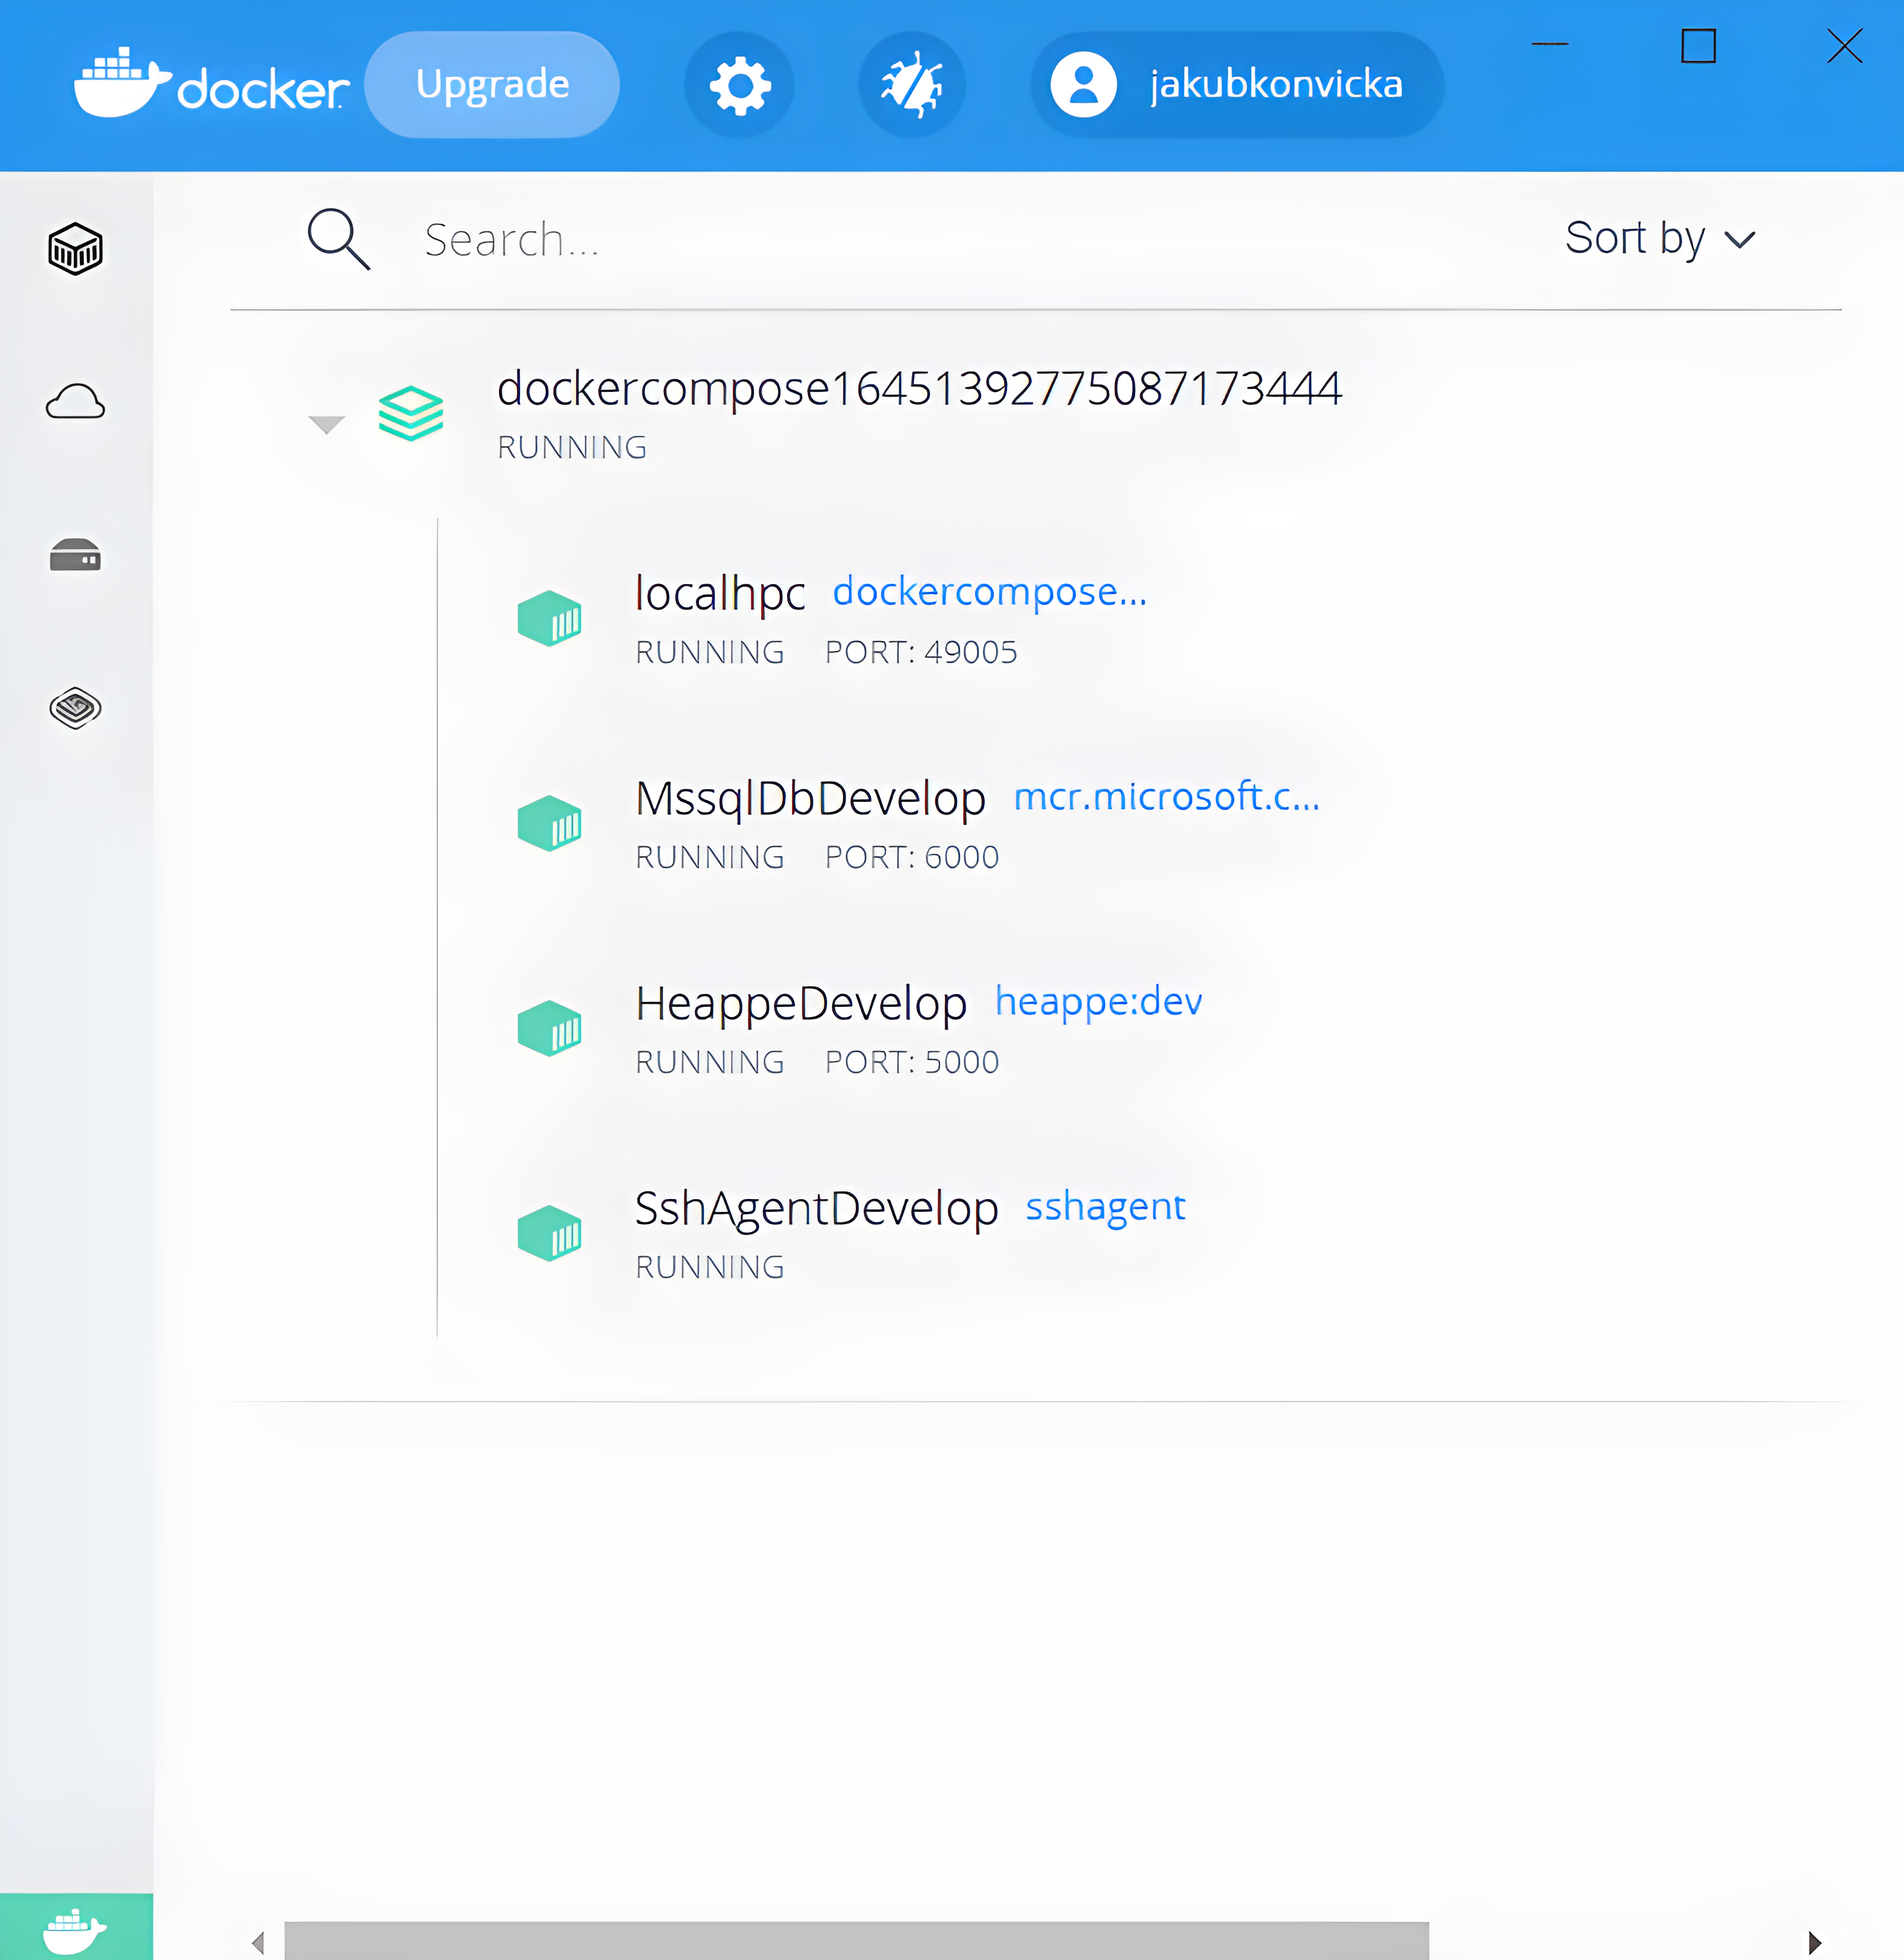
\includegraphics[width=0.8\textwidth]{Figures/dockerdesktophq.jpg}
	\caption{Ukázka aplikace Docker Desktop se spuštěným kontejnerem}
    \label{fig:WritingThesis}
\end{figure}

\chapter{Příklad specifikace testovacího plánu pro Robot Framework}
\lstinputlisting[language=bash, caption={Specifikace Robot Framework testu}]{SourceCodes/robot-framework-demo.txt}



\chapter{Robot Framework - výstup testu}\label{chapter:robot-framework-local-tests}

\begin{figure}[!h]
	\centering
	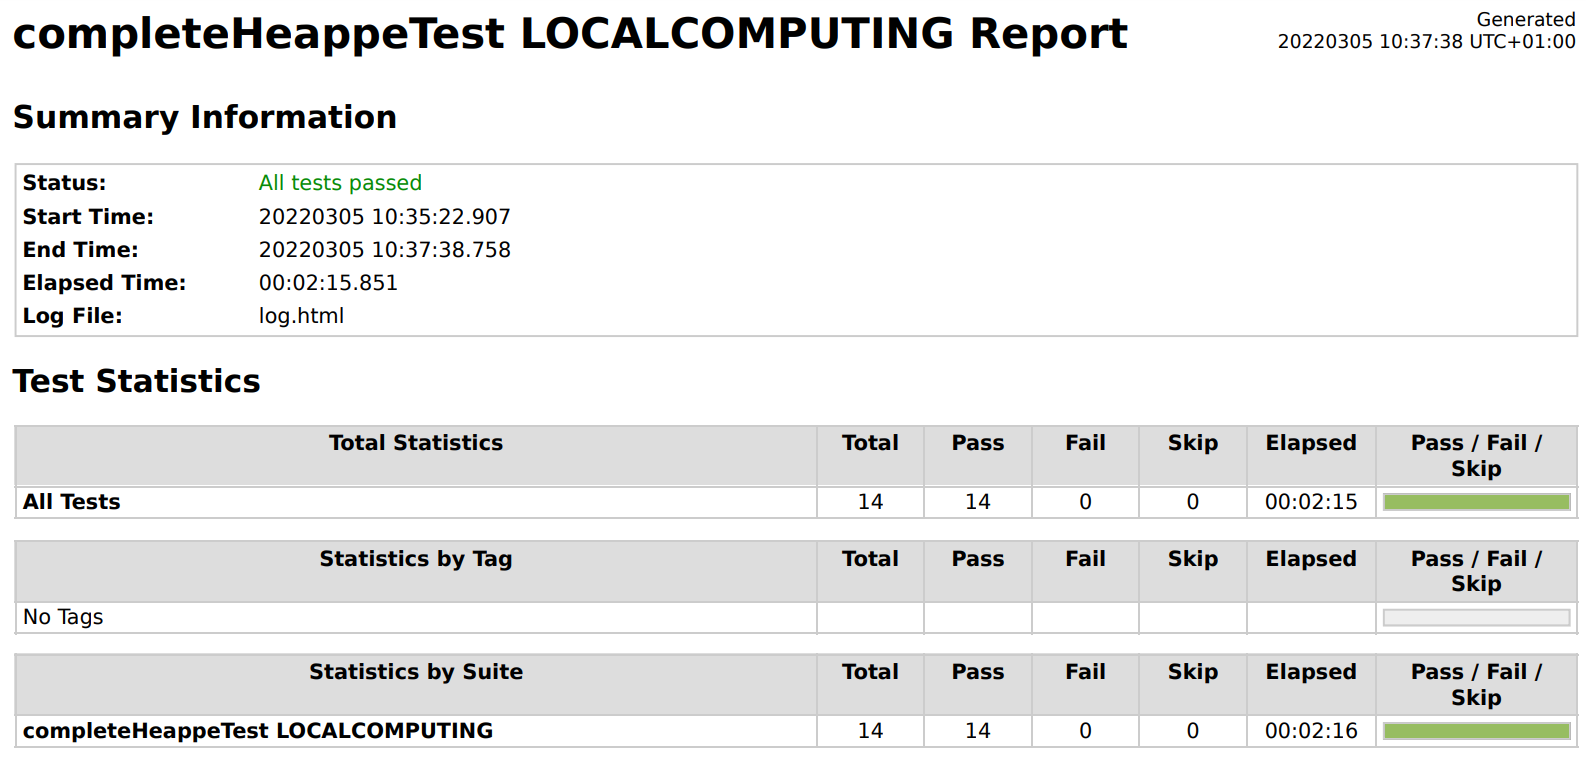
\includegraphics[width=1\textwidth]{Figures/robot-report.png}
	\caption{Report Robot Frameworku}
    \label{fig:robotFrameworkReport}
\end{figure}

\begin{figure}[!h]
	\centering
	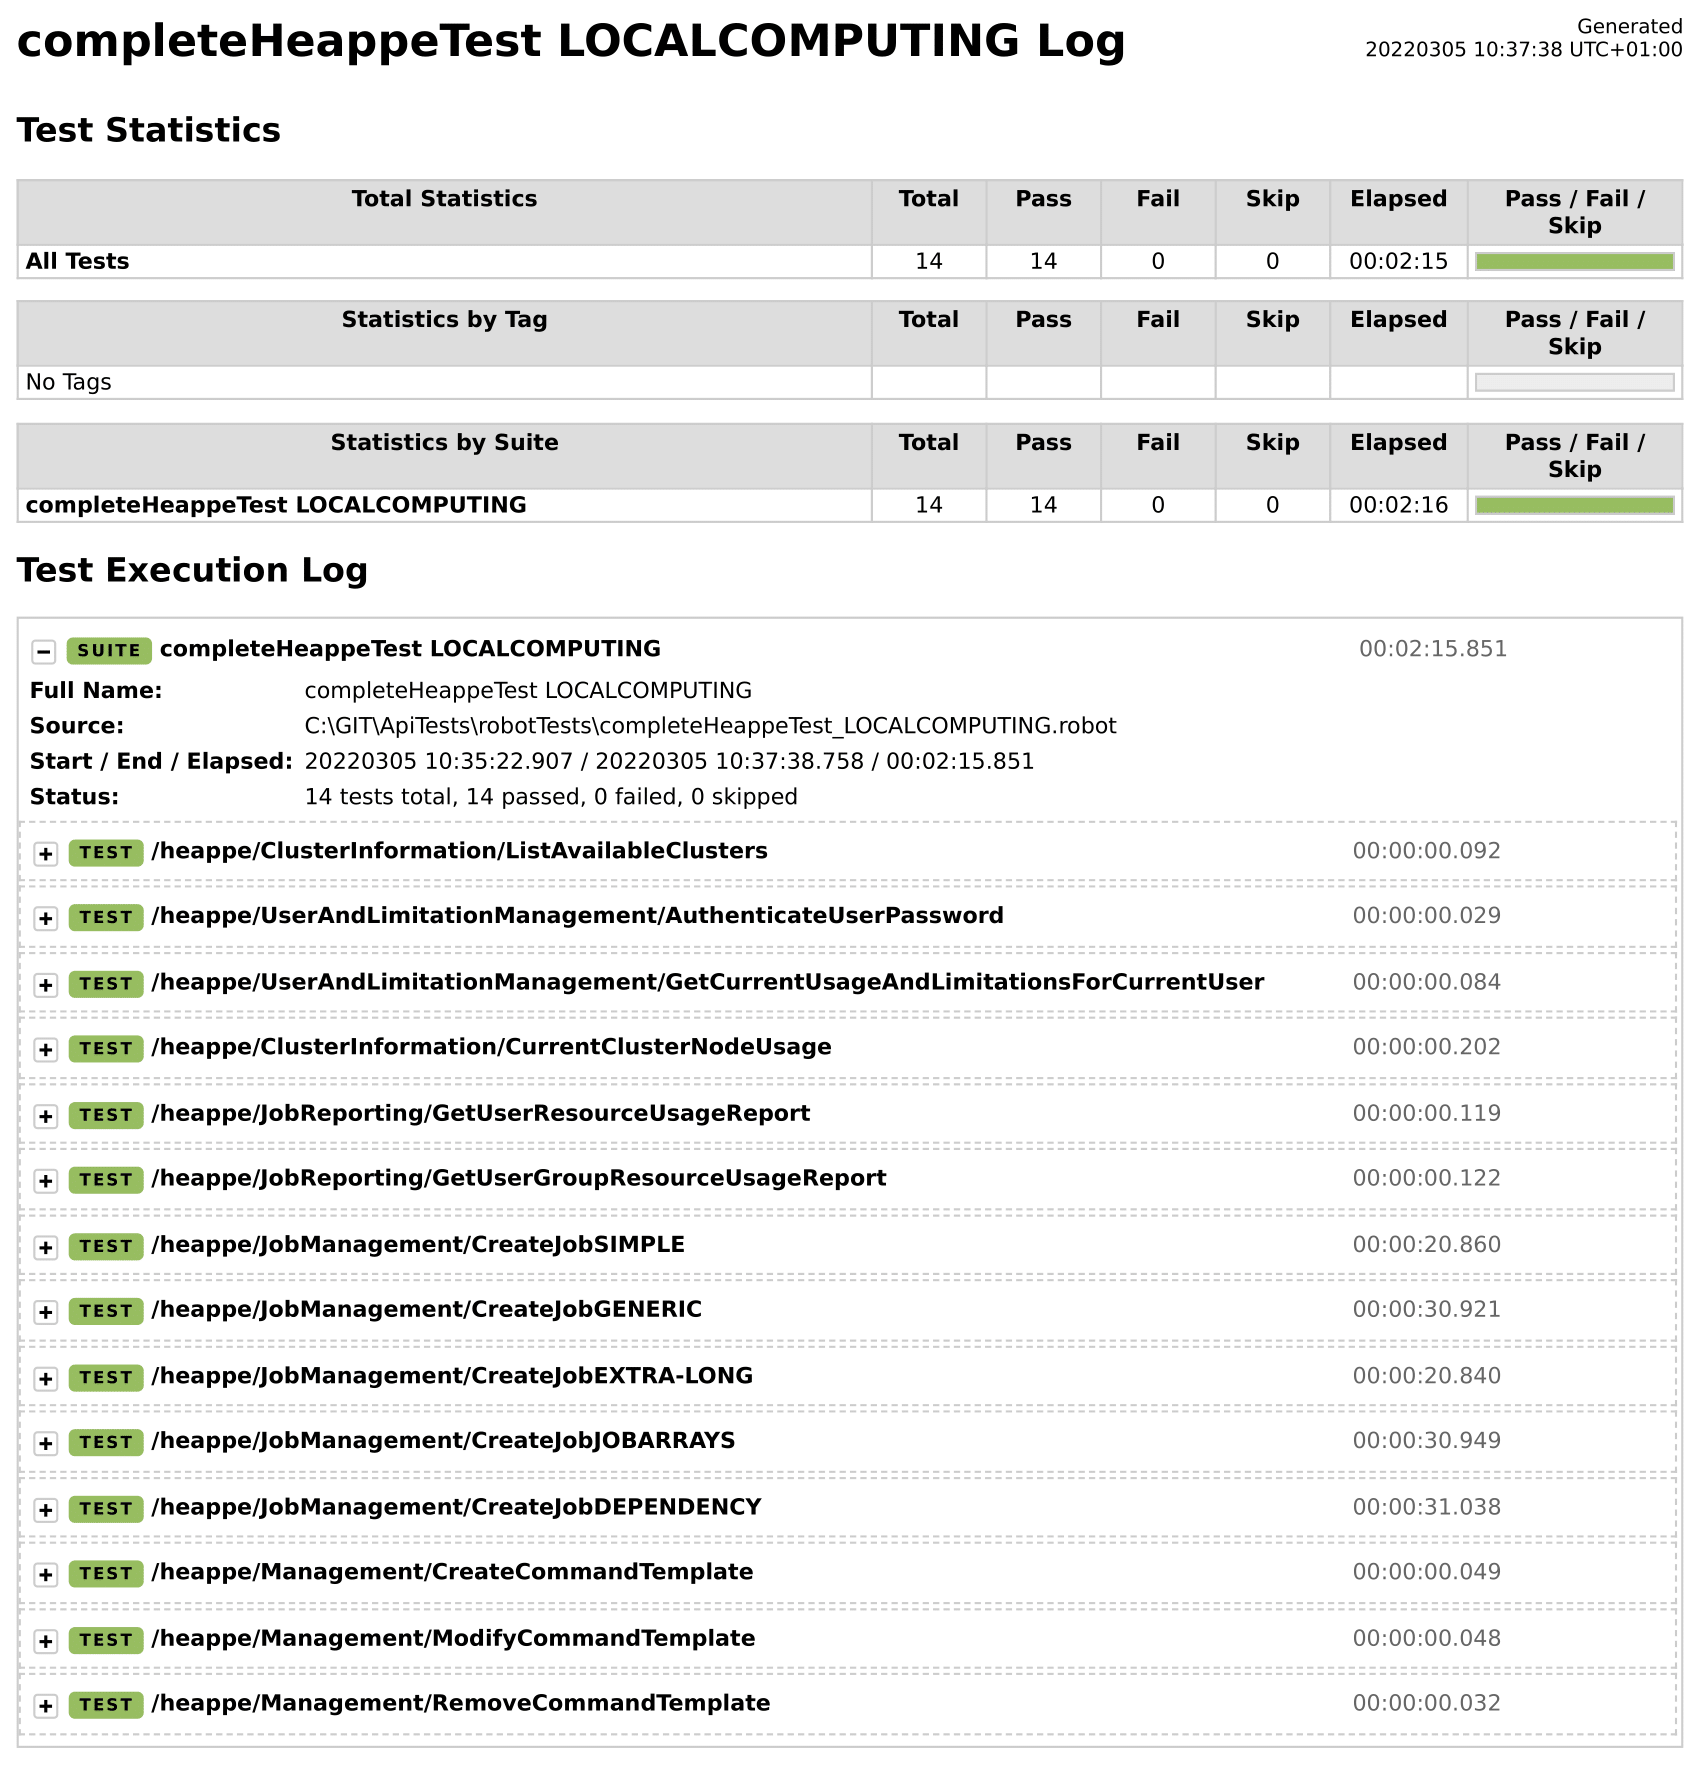
\includegraphics[width=1\textwidth]{Figures/robot-log.png}
	\caption{Log Robot Frameworku}
    \label{fig:robotFrameworkLog}
\end{figure}



\chapter{Výstup testování přenosu souborů}\label{manual-tests}

\lstinputlisting[caption={Log aplikace provádějící test HEAppE funkcionalit}]{SourceCodes/heappe-test-app-log.txt}


\newpage
\lstinputlisting[caption={Log HEAppE Middleware - FileTransfer}]{SourceCodes/heappe-log-scp.txt}

\lstinputlisting[caption={Vylistování adresáře na lokálním HPC clusteru s výběrem souboru a.txt}]{SourceCodes/ls-grep-a.txt}




\end{document}
